% =============================================================================
% گزارش پروژه کارشناسی — دانشگاه شهرکرد
% قالب: XeLaTeX + xepersian
%   فارسی:   XB Zar (خانوادهٔ zar) اندازهٔ 13، فاصلهٔ خطوط 0.9cm
%   انگلیسی: Times (Liberation Serif به‌عنوان جایگزین متریک، و mathptmx
%            برای فرمول‌ها به‌صورت ایتالیک)
%   حاشیه‌ها: راست 3cm، چپ 2.5cm، پایین 2.5cm، بالا 3cm
%            (6cm برای صفحهٔ نخست هر فصل)
% =============================================================================
\documentclass[12pt,a4paper]{report}

\usepackage{mathptmx}   % Times برای متن/فرمول‌های لاتین (فرمول‌ها ایتالیک)
\usepackage{amsmath,amssymb}

\usepackage[a4paper]{geometry}
\geometry{top=3cm,bottom=2.5cm,left=2.5cm,right=3cm}

\usepackage{graphicx}
\usepackage{microtype}
\emergencystretch=3em
\tolerance=1000

% For breaking long code/URL strings
\usepackage[hyphens]{url}
\Urlmuskip=0mu plus 1mu
\usepackage{xurl}

\usepackage{booktabs}
\usepackage{array}
\usepackage{caption}
\usepackage{float}
\usepackage{enumitem}
\usepackage{xcolor}

% نمودارهای معماری: همهٔ شکل‌ها به‌صورت متن (TikZ) نگهداری می‌شوند تا مانند
% کد، نسخه‌پذیری، diff و بازبینی داشته باشند؛ نه تصویر خروجی ابزار بیرونی.
\usepackage{tikz}
\usetikzlibrary{arrows.meta,positioning,fit,calc,backgrounds}
\tikzset{
  box/.style={draw=black!60, rounded corners=1.5pt, align=center, inner sep=3pt,
              minimum height=8mm, fill=blue!8, font=\footnotesize},
  data/.style={draw=black!60, rounded corners=1.5pt, align=center, inner sep=3pt,
               minimum height=8mm, fill=orange!18, font=\footnotesize},
  ext/.style={draw=black!60, dashed, rounded corners=1.5pt, align=center, inner sep=3pt,
              minimum height=8mm, fill=gray!10, font=\footnotesize},
  usr/.style={draw=black!60, rounded corners=1.5pt, align=center, inner sep=3pt,
              minimum height=8mm, fill=yellow!25, font=\footnotesize},
  proc/.style={draw=black!60, rounded corners=1.5pt, align=center, inner sep=3pt,
               minimum height=8mm, fill=green!14, font=\footnotesize},
  art/.style={draw=black!60, rounded corners=1.5pt, align=center, inner sep=3pt,
              minimum height=8mm, fill=violet!14, font=\footnotesize},
  lane/.style={font=\small\bfseries, align=center},
  w/.style={text width=#1},
  arr/.style={-{Stealth[length=2.4mm]}, line width=0.7pt, draw=black!70},
  arrd/.style={arr, dashed},
  lbl/.style={font=\scriptsize, align=center, fill=white, inner sep=1.2pt},
}

\usepackage{hyperref}
\hypersetup{
  colorlinks=true,
  linkcolor=blue!50!black,
  urlcolor=blue!50!black,
  citecolor=blue!50!black,
  hyperfootnotes=false,
  pdftitle={تشخیص متن تولیدشده توسط هوش مصنوعی در زبان فارسی},
  pdfauthor={احسان ترابی فرسانی},
}
\newcommand{\code}[1]{\texttt{#1}}
\DeclareRobustCommand{\en}[1]{\lr{#1}}

% ---------------------------------------------------------------------------
% اندازهٔ متن بدنه: 13pt با فاصلهٔ خطوط 0.9cm (~25.5pt)
% ---------------------------------------------------------------------------
\makeatletter
\renewcommand\normalsize{\@setfontsize\normalsize{13pt}{25.54pt}}
\renewcommand\small{\@setfontsize\small{11.5pt}{16.5pt}}
\renewcommand\footnotesize{\@setfontsize\footnotesize{10.5pt}{14.5pt}}
\normalsize

% سر فصل: علاوه بر حاشیهٔ بالای 3cm صفحه‌گزینه، 30mm فضای اضافی تا عنوان
% فصل => حاشیهٔ بالای مؤثر 6cm در صفحهٔ نخست هر فصل
\renewcommand\@makechapterhead[1]{%
  {\parindent\z@
    \vspace*{30mm}%
    \ifnum \c@secnumdepth >\m@ne
      \if@mainmatter
        {\LARGE\bfseries \@chapapp~\thechapter}%
        \par\nobreak
        \vskip 12\p@
      \fi
    \fi
    \interlinepenalty\@M
    {\huge\bfseries #1}%
    \par\nobreak
    \vskip 24\p@
  }}
\renewcommand\@makeschapterhead[1]{%
  {\parindent\z@
    \vspace*{30mm}%
    \interlinepenalty\@M
    {\huge\bfseries #1}%
    \par\nobreak
    \vskip 24\p@
  }}
\makeatother

\setcounter{secnumdepth}{2}  % شماره‌گذاری تا زیربخش x.y.z
\setcounter{tocdepth}{1}     % فهرست: فصل‌ها و بخش‌ها

% ---------------------------------------------------------------------------
% فونت‌ها
% ---------------------------------------------------------------------------
\usepackage{xepersian}
\settextfont[
  Path = /home/ehsan/.fonts/truetype/XBZar/Zar/,
  Extension = .ttf,
  UprightFont = *,
  % نکته: قلم Bold واقعی XB Zar (فایل *Bd) نیم‌فاصله (U+200C) را به‌صورت
  % خط عمودی مرئی رسم می‌کند؛ بولد مصنوعی از قلم Regular این ایراد را ندارد.
  AutoFakeBold = 2.5,
]{XB Zar}
% Times New Roman روی این سامانه نصب نیست؛ Liberation Serif نزدیک‌ترین
% جایگزین متریک آن است.
\setlatintextfont{Liberation Serif}
\setdigitfont[
  Path = /home/ehsan/.fonts/truetype/XBZar/Zar/,
  Extension = .ttf,
  UprightFont = *,
  AutoFakeBold = 2.5,
]{XB Zar}

\renewcommand{\chaptername}{فصل}
\renewcommand{\appendixname}{پیوست}
\renewcommand{\contentsname}{فهرست}
\renewcommand{\bibname}{مراجع}

% بلوک‌های verbatim چپ‌به‌راست: علاوه بر تغییر جهت پاراگراف، سازوکار
% درون‌کاری نویسه‌های xepersian نیز خاموش می‌شود تا دنباله‌هایی مانند
% 0.02 یا 0.0.0.0:8000 در چیدمان دوجهته جابه‌جا نشوند.
\newenvironment{LTRverb}
  {\begin{LTR}\XeTeXinterchartokenstate=0}
  {\end{LTR}}

% آرم دانشگاه: در صورت قرارگرفتن logo.png یا logo.jpg در پوشهٔ report،
% به‌طور خودکار استفاده می‌شود؛ در غیر این صورت کادر جای‌نگه‌دار نمایش
% داده می‌شود.
\newcommand{\universitylogo}{%
  \IfFileExists{logo.png}%
    {
\includegraphics[width=3.2cm]{logo.png}}%
    {\IfFileExists{logo.jpg}%
      {\includegraphics[width=3.2cm]{logo.jpg}}%
      {\fbox{\parbox[c][3cm][c]{3.8cm}{\centering جای آرم\\دانشگاه}}}}%
}

\begin{document}

% شماره‌گذاری متن پیشین (تشکر، فهرست، چکیده) با حروف ابجد و بدون شمارهٔ
% نمایان؛ متن اصلی از ۱ شروع می‌شود.
\pagestyle{empty}
\pagenumbering{abjad}

% =============================================================================
% ۱) برگ نخست: سفید
% =============================================================================
\thispagestyle{empty}
\null
\clearpage

% =============================================================================
% ۲) بسم الله الرحمن الرحیم (وسط صفحه)
% =============================================================================
\thispagestyle{empty}
\vspace*{\fill}
\begin{center}
  {\huge بِسْمِ اللهِ الرَّحْمٰنِ الرَّحِیم}
\end{center}
\vspace*{\fill}
\clearpage

% =============================================================================
% ۳) صفحهٔ عنوان: آرم دانشگاه، عنوان پروژه، استاد راهنما، دانشجو، ماه ارائه
% =============================================================================
\thispagestyle{empty}
\begin{center}
  \vspace*{5mm}
  \universitylogo\\[7mm]
  {\Large دانشگاه شهرکرد}\\[20mm]
  {\huge\bfseries تشخیص متن تولیدشده توسط هوش مصنوعی در زبان فارسی}\\[6mm]
  {\large معماری سامانه، روش‌شناسی یادگیری ماشین و یادگیری عمیق، و تحلیل خطا}\\[22mm]
  {\large\bfseries استاد راهنما}\\[2mm]
  {دکتر ــــــــــــــــــــــــــــــــــــ}\\[12mm]
  {\large\bfseries نگارنده}\\[2mm]
  {احسان ترابی فرسانی}\\[\fill]
  {\large ماه ارائه: مهر ۱۴۰۵}\\[8mm]
\end{center}
\clearpage

% شروع شمارش ابجدِ متن پیشین از صفحهٔ تشکر (صفحات ۱ تا ۳ شماره نمی‌گیرند)
\setcounter{page}{1}

% =============================================================================
% ۴) تشکر و قدردانی
% =============================================================================
\phantomsection
\addcontentsline{toc}{chapter}{تشکر و قدردانی}
\chapter*{تشکر و قدردانی}
از استاد راهنمای محترم که با راهنمایی‌های ارزشمند خود مسیر این پروژه را
روشن ساختند، و از پژوهشگران و تیم‌های متن‌باز — به‌ویژه سازندگان کتابخانه‌های
\en{scikit-learn}، \en{PyTorch}، \en{transformers} و \en{shekar}، و
تیم \en{HooshvareLab} برای انتشار مدل زبانی \en{GPT-2} فارسی — صمیمانه
سپاس‌گزارم. همچنین از ارائه‌دهندگان سرویس‌های زبانی که در گردآوری مجموعه
دادهٔ این پروژه به‌کار گرفته شدند، قدردانی می‌شود.

% =============================================================================
% ۵) فهرست
% =============================================================================
\tableofcontents

% =============================================================================
% چکیده
% =============================================================================
\phantomsection
\addcontentsline{toc}{chapter}{چکیده}
\chapter*{چکیده}
این گزارش سامانه‌ای را شرح می‌دهد که تشخیص می‌دهد یک متن فارسی را انسان
نوشته است یا یک مدل زبانی. روی یک مجموعه‌دادهٔ متوازن، هفت مدل پایهٔ
طبقه‌بندی دودویی آموزش دیده‌اند: پنج مدل یادگیری ماشین کلاسیک روی ویژگی‌های
\en{TF-IDF} به‌همراه چهار ویژگی سبک‌شناسی دست‌ساز (آنتروپی، تنوع طول جمله،
تکرار سه‌گرم و انسجام میان‌جمله‌ای)، یک \en{BiLSTM} با \en{embedding}
آموخته‌شده از ابتدا، و \en{GPT-2} فارسی فاین‌تیون‌شده. متن‌های کلاس هوش
مصنوعی را خط‌لوله‌ای جداگانه با هفتاد مدل زبانی از نُه ارائه‌دهندهٔ \en{API}
و پنج سبک نوشتاری تولید کرده است؛ این مجموعه‌داده با فرادادهٔ کامل و مجوز
\en{Apache 2.0} در \en{Hugging Face} منتشر شده است.

گزارش ابتدا خط‌لولهٔ پیش‌پردازش، استخراج ویژگی، معماری ریاضی هر مدل،
روش تنظیم هایپرپارامتر و معیارهای ارزیابی را توضیح می‌دهد، سپس خطای
نسخهٔ نخست مدل‌ها را ریشه‌یابی می‌کند: ارقام $F_1$ بالای $0.99$ روی مجموعهٔ
آزمون ثابت با خطای محسوس روی متن واقعی هم‌خوان نبودند، و علت نبود تنظیم
هایپرپارامتر، فضای ویژگی نامناسب و نشت داده در انتخاب مدل بود. خط‌لولهٔ دوم
روی \en{Google Colab} هر سه ایراد را برطرف کرده و نتایج عددی آن در
جدول~\ref{tab:results-v2} آمده است.

تحلیل خطای \en{BiLSTM} نشان داد ضعف اصلی این مدل پیاده‌سازی نیست، بلکه
حساسیت آن به تغییر توزیف میان سبک نوشتاری دادهٔ آموزش و متن کاربران است.
دو ماژول تازه از همین یافته بیرون آمده‌اند: \en{ParsBERT} به‌عنوان رمزگذار
دوسویهٔ پیش‌آموزش‌دیدهٔ فارسی، و یک لایهٔ تصمیم «سیستم-یک» به سبک \en{JEV}
که به‌جای یک احتمال، سه پاسخ نوع‌بندی‌شده (انتخاب، امتیاز، نیاز به بازبینی)
برمی‌گرداند. \en{ParsBERT} روی \en{Google Colab} بازآموزی، در سرور مستقر و
ارقامش به جدول~\ref{tab:results-v2} افزوده شده است؛ لایهٔ تصمیم سیستم-یک بر
همین رمزگذار فاین‌تیون‌شده استوار است، هدف‌های نرم آن از دسته‌بند
\en{GPT-2} فاین‌تیون‌شده تقطیر می‌شود و ارقام آموزشش در
بخش~\ref{sec:jev} آمده است. در کنار این دو، یک شاخص سرگشتگی بدون‌آموزش
از مدل زبانی خام به سرویس افزوده شده است؛ بررسی تجربی آن
(بخش~\ref{sec:perplexity-signal}) جهت سیگنال را روی این مجموعه وارونه
نشان می‌دهد و به همین دلیل تنها به‌عنوان شاخص نمایشی مانده است.

\vspace{4mm}
\noindent\textbf{کلیدواژه‌ها:} تشخیص متن ماشینی، پردازش زبان طبیعی فارسی،
\en{TF-IDF}، ویژگی‌های سبک‌شناسی، \en{BiLSTM}، ترنسفورمر، فاین‌تیون، تقطیر
دانش، بیش‌برازش، تغییر توزیع

% =============================================================================
% ۶) متن اصلی — فصل‌بندی بر اساس کار انجام‌شده
% =============================================================================
\clearpage
\pagestyle{plain}
\pagenumbering{arabic}

% -----------------------------------------------------------------------------
\chapter{مقدمه}
% -----------------------------------------------------------------------------

\section{انگیزه و اهمیت مسئله}
در دسترس قرارگرفتن ابزارهای تولید متن، مسئلهٔ تشخیص اینکه یک قطعه متن را
انسان نوشته است یا یک مدل زبانی تولید کرده، به مسئله‌ای روزمره در آموزش
(تشخیص تقلب در تکالیف)، نشر محتوا، اعتبارسنجی خبر و تعدیل محتوا تبدیل شده
است. بیشتر ابزارهای تجاری این حوزه برای انگلیسی بهینه شده‌اند و روی فارسی
افت محسوسی دارند؛ تفاوت صرف واژگان، نیم‌فاصله (\en{ZWNJ})، دستور زبان و
کمبود منابع پیش‌آموزش، همگی در این افت نقش دارند. این پروژه برای فارسی یک
سامانهٔ اختصاصی می‌سازد: چند خانوادهٔ مدل — از خطی ساده تا ترنسفورمر عمیق —
روی یک مجموعه‌دادهٔ متوازن فارسی آموزش می‌بینند و از طریق یک \en{API} و یک
رابط کاربری وب در دسترس قرار می‌گیرند.

\section{چالش‌های خاص زبان فارسی}
پردازش متن فارسی چند چالش فنی دارد که مستقیماً روی طراحی خط‌لولهٔ
پیش‌پردازش این پروژه اثر گذاشته‌اند:
\begin{itemize}[rightmargin=1em]
  \item \textbf{اختلاط حروف عربی و فارسی:} حروفی مانند «ی/ي» و «ک/ك» در
    منابع مختلف به هر دو صورت عربی و فارسی نوشته می‌شوند و بدون یکسان‌سازی،
    یک واژه به دو توکن متفاوت تبدیل می‌شود.
  \item \textbf{نیم‌فاصله:} فاصله‌گذاری نادرست یا نبود نیم‌فاصله در واژه‌های
    مرکب (مانند «می‌روم» در برابر «می روم» یا «میروم») واحدهای واژگانی را
    جابه‌جا می‌کند.
  \item \textbf{صرف پیچیده:} فعل‌ها و اسم‌های فارسی صرف‌های متعددی دارند و
    بدون ریشه‌یابی، حجم واژگان مدل‌های کیسه‌واژه (\en{bag-of-words}) بالا و
    پراکندگی (\en{sparsity}) ویژگی‌ها شدید می‌شود.
  \item \textbf{کمبود منابع پیش‌آموزش‌دیده:} برخلاف انگلیسی، مدل‌های زبانی
    پیش‌آموزش‌دیدهٔ فارسی معدودتر و کوچک‌ترند. این پروژه از
    \en{HooshvareLab/gpt2-fa} — یک \en{GPT-2} با ۱۲۴ میلیون پارامتر که روی
    پیکرهٔ فارسی آموزش دیده — و از \en{ParsBERT} استفاده می‌کند.
\end{itemize}

\section{نمای کلی سامانه}
\label{sec:overview}
شکل~\ref{fig:overview} سه لایهٔ اصلی سامانه را در یک نما نشان می‌دهد؛ جهت
جریان از راست به چپ و مطابق جهت خواندن است. لایهٔ نخست، داده را می‌سازد
(بخش‌های~\ref{sec:data-collection} و~\ref{sec:split}): متن هوش‌مصنوعی با
تنوع عمدی چهارگانه (ارائه‌دهنده و مدل، سبک، موضوع، پارامتر نمونه‌برداری)
گردآوری و با متن انسانی وبلاگ‌ها توازن داده می‌شود؛ سپس تفکیک سه‌گانهٔ
آموزش/اعتبارسنجی/آزمون با بذر ثابت ساخته می‌شود. لایهٔ دوم، نُه مدل را در
چهار خانوادهٔ الگوریتمی آموزش می‌دهد: پنج مدل کلاسیک روی فضای
\en{TF-IDF} و ویژگی‌های سبک‌شناسی، \en{BiLSTM}، \en{GPT-2} فاین‌تیون‌شده
(که نقش معلم تقطیر را نیز برای لایهٔ تصمیم \en{JEV} بر عهده دارد)،
\en{ParsBERT} فاین‌تیون‌شده و سرهای تصمیم \en{JEV}. خروجی این لایه
چک‌پوینت‌های خودکفا به‌همراه پروندهٔ \texttt{models.json} است. لایهٔ سوم
آن چیزی است که کاربر می‌بیند: سرویس \en{FastAPI} که بارگذاری و استنتاج را
بر اساس فیلد \texttt{runtime} اعزام می‌کند (بخش~\ref{sec:service-arch}) و
رابط وب \en{Next.js} که در سه حالت محلی، آنلاین و مقایسه کار می‌کند
(بخش~\ref{sec:online-systemone}).

\begin{figure}[H]
\centering
\resizebox{\textwidth}{!}{%
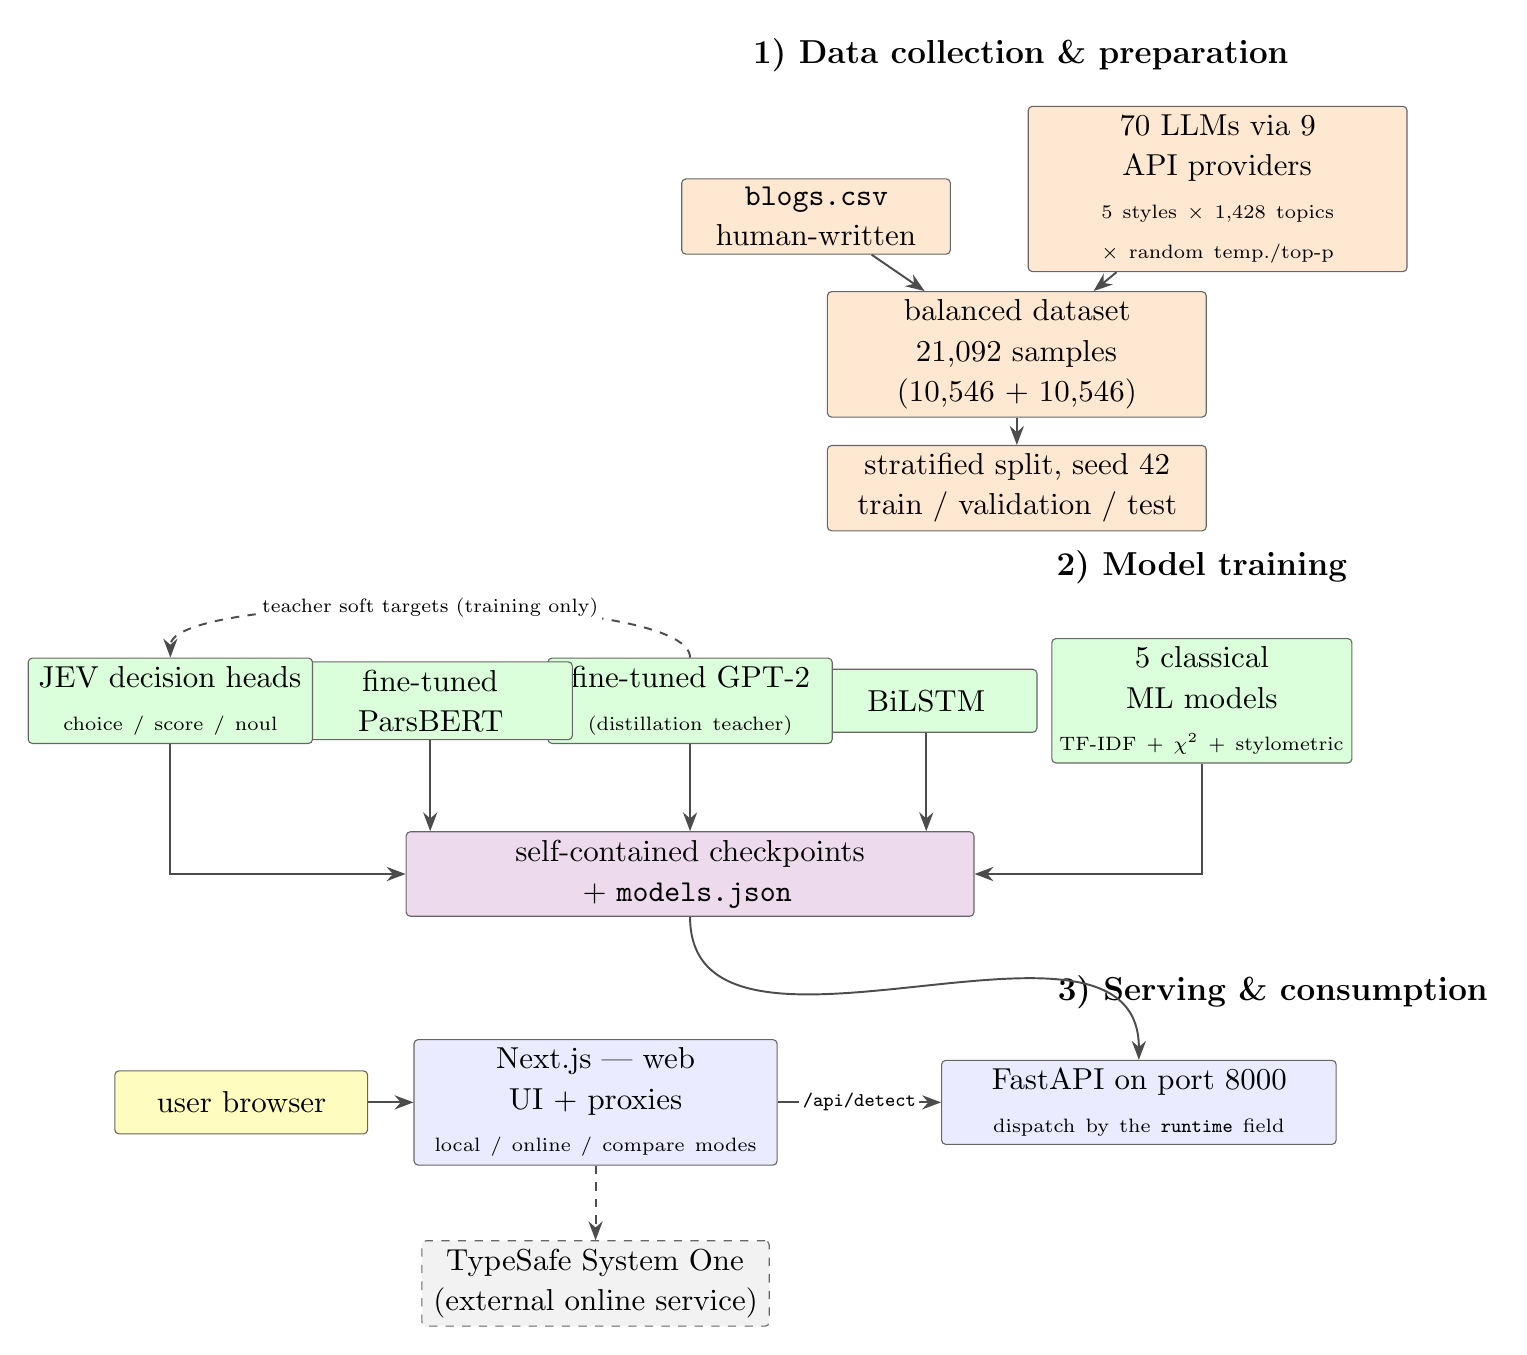
\begin{tikzpicture}
  % ---------- Layer 1: data ----------
  \node[lane] at (-2.5,1.7) {\en{1) Data collection \& preparation}};
  \node[data, w=4.6cm] (collect) at (0,0)
      {\en{70} LLMs via \en{9} API providers\\[1pt]
       \scriptsize \en{5} styles $\times$ \en{1,428} topics $\times$ random temp./top-p};
  \node[data, w=3.2cm] (blogs) at (-5.1,-0.35)
      {\texttt{blogs.csv}\\human-written};
  \node[data, w=4.6cm] (dataset) at (-2.55,-2.1)
      {balanced dataset\\\en{21,092} samples (\en{10,546} + \en{10,546})};
  \node[data, w=4.6cm] (split) at (-2.55,-3.8)
      {stratified split, seed \en{42}\\train / validation / test};
  \draw[arr] (collect) -- (dataset);
  \draw[arr] (blogs) -- (dataset);
  \draw[arr] (dataset) -- (split);
  % ---------- Layer 2: training ----------
  \node[lane] at (-0.2,-4.8) {\en{2) Model training}};
  \node[proc, w=3.6cm] (m1) at (-0.2,-6.5)
      {\en{5} classical ML models\\[1pt]\scriptsize \en{TF-IDF} + $\chi^2$ + stylometric};
  \node[proc, w=2.6cm] (m2) at (-3.7,-6.5) {\en{BiLSTM}};
  \node[proc, w=3.4cm] (m3) at (-6.7,-6.5)
      {\en{fine-tuned GPT-2}\\[1pt]\scriptsize (distillation teacher)};
  \node[proc, w=3.4cm] (m4) at (-10.0,-6.5) {fine-tuned \en{ParsBERT}};
  \node[proc, w=3.4cm] (m5) at (-13.3,-6.5)
      {\en{JEV} decision heads\\[1pt]\scriptsize choice / score / noul};
  \draw[arrd] (m3.north) .. controls (-6.7,-5.1) and (-13.3,-5.1) ..
      node[lbl] {teacher soft targets (training only)} (m5.north);
  \node[art, w=7.0cm] (art1) at (-6.7,-8.7)
      {self-contained checkpoints\\+ \texttt{models.json}};
  \draw[arr] (m2.south) -- (m2.south |- art1.north);
  \draw[arr] (m3.south) -- (m3.south |- art1.north);
  \draw[arr] (m4.south) -- (m4.south |- art1.north);
  \draw[arr] (m1.south) |- (art1.east);
  \draw[arr] (m5.south) |- (art1.west);
  % ---------- Layer 3: serving ----------
  \node[lane] at (0.7,-10.2) {\en{3) Serving \& consumption}};
  \node[box, w=4.8cm] (s1) at (-1.0,-11.6)
      {\en{FastAPI} on port \en{8000}\\[1pt]\scriptsize dispatch by the \texttt{runtime} field};
  \node[box, w=4.4cm] (s2) at (-7.9,-11.6)
      {\en{Next.js} — web UI + proxies\\[1pt]\scriptsize local / online / compare modes};
  \node[usr, w=3.0cm] (s3) at (-12.4,-11.6) {user browser};
  \node[ext, w=4.2cm] (s4) at (-7.9,-13.9)
      {\en{TypeSafe System One} (external online service)};
  \draw[arr] (art1.south) to[out=-90,in=90] (s1.north);
  \draw[arr] (s2.east) -- node[lbl] {\texttt{/api/detect}} (s1.west);
  \draw[arr] (s3) -- (s2);
  \draw[arrd] (s2.south) -- (s4.north);
\end{tikzpicture}}%
\caption{نمای کلی سه‌لایهٔ سامانه: گردآوری داده، آموزش و سرویس‌دهی. جریان از
راست به چپ خوانده می‌شود؛ پیکان نقطه‌چین میان \en{GPT-2} و \en{JEV} تنها در
زمان آموزش (تقطیر) فعال است و سرویس بیرونی \en{TypeSafe} اختیاری است.}
\label{fig:overview}
\end{figure}

% -----------------------------------------------------------------------------
\chapter{مجموعه داده}
% -----------------------------------------------------------------------------

\section{منابع داده}
مجموعه دادهٔ نهایی از ترکیب دو منبع ساخته شده است:
\begin{itemize}[rightmargin=1em]
  \item \texttt{persian\_ai\_generated\_final.csv}: متن‌های تولیدشده توسط
    مدل‌های زبانی هوش مصنوعی (برچسب مثبت، \en{aiGenerated=1}).
  \item \texttt{blogs.csv}: متن‌های وبلاگ نوشته‌شده توسط انسان (برچسب منفی،
    \en{aiGenerated=0}).
\end{itemize}
برای جلوگیری از عدم توازن کلاس (\en{class imbalance})، از مجموعهٔ
\texttt{blogs.csv} به تعداد نمونه‌های کلاس هوش مصنوعی نمونه‌برداری تصادفی
انجام شده است. مجموعهٔ نهایی (\texttt{processedDataset.csv}) شامل
$21{,}092$ نمونه است که دقیقاً به دو کلاس $10{,}546$ تایی تقسیم می‌شود
(جدول~\ref{tab:dataset}).

\begin{table}[H]
\centering
\caption{ترکیب مجموعه داده}
\label{tab:dataset}
\begin{tabular}{lr}
\toprule
\textbf{کلاس} & \textbf{تعداد نمونه} \\
\midrule
انسان (\en{aiGenerated=0}) & $10{,}546$ \\
هوش مصنوعی (\en{aiGenerated=1}) & $10{,}546$ \\
\midrule
\textbf{مجموع} & $21{,}092$ \\
\bottomrule
\end{tabular}
\end{table}

\section{روش گردآوری بخش هوش‌مصنوعی داده}
\label{sec:data-collection}
بخش هوش‌مصنوعی مجموعه داده (\texttt{persian\_ai\_generated\_final.csv}) را
خط‌لولهٔ گردآوری جداگانهٔ پروژهٔ \en{AITextGeneration} تولید کرده است. این
خط‌لوله بر تنوع تأکید دارد، چون هدف پروژه یادگیری یک ویژگی عمومی «متن
تولیدشده توسط هوش مصنوعی» است، نه الگوهای سبکی یک مدل خاص:
\begin{itemize}[rightmargin=1em]
  \item \textbf{چندارائه‌دهندگی و چندمدلی:} درخواست‌ها به‌صورت هم‌زمان
    (\en{ThreadPoolExecutor}) به $9$ ارائه‌دهندهٔ \en{API} مختلف
    (\en{OpenRouter}، \en{NVIDIA}، و چند نقطهٔ پایانی سازگار با \en{OpenAI})
    ارسال می‌شوند که در مجموع به $70$ مدل زبانی متفاوت از خانواده‌های
    \en{GPT}، \en{Claude}، \en{Gemini}/\en{Gemma}، \en{DeepSeek}،
    \en{Llama}، \en{Qwen}، \en{Nemotron} و دیگر مدل‌های \en{open-weight}
    دسترسی می‌دهند؛ برای هر نمونه، ارائه‌دهنده و مدل به‌صورت تصادفی انتخاب
    می‌شوند.
  \item \textbf{تنوع سبک نوشتاری:} هر درخواست یکی از $5$ دستورالعمل سیستمی
    (\en{system prompt}) از پیش طراحی‌شده را دریافت می‌کند: مقالهٔ رسمی
    (\en{formal\_essay})، پست وبلاگی محاوره‌ای (\en{conversational\_blog})،
    پاسخ پرسش‌وپاسخی گام‌به‌گام (\en{qa\_explainer})، متن انتقادی/استدلالی
    (\en{opinion\_critical})، و خلاصهٔ ساختاریافته (\en{summary\_overview}).
  \item \textbf{تنوع موضوعی:} موضوع هر درخواست از میان $1{,}428$ موضوع
    یکتای فارسی—در حوزه‌های علم و فناوری، اقتصاد، سلامت، فلسفه، هنر و
    محیط‌زیست—به‌طور تصادفی انتخاب می‌شود.
  \item \textbf{تصادفی‌سازی پارامترهای نمونه‌برداری:} برای هر درخواست، دما
    (\en{temperature}) از بازهٔ $[0.30,\ 0.95]$ و \en{top-p} از بازهٔ
    $[0.80,\ 1.00]$ به‌طور یکنواخت نمونه‌برداری می‌شود تا سرگشتگی
    (\en{perplexity}) و روانی متن تولیدشده در طیف وسیعی پراکنده باشد، نه
    فقط حول یک تنظیم پیش‌فرض ثابت.
\end{itemize}
این چهار محور — ارائه‌دهنده و مدل، سبک، موضوع، پارامتر نمونه‌برداری — با
هدف کاهش ریسک یادگیری \textbf{اثرانگشت یک مدل خاص} به‌جای ویژگی‌های عمومی
متن ماشینی طراحی شده‌اند. با این حال، بخش~\ref{sec:bilstm-error-analysis}
نشان می‌دهد که این تنوع کافی نبوده و در تعمیم‌پذیری خارج از توزیع همچنان
شکاف قابل‌اندازه‌گیری باقی مانده است.

بخش هوش مصنوعی این مجموعه داده، با فرادادهٔ کامل ردیابی (مدل، ارائه‌دهنده،
سبک، دما، \en{top-p})، با مجوز \en{Apache 2.0} در \en{Hugging Face Datasets}
منتشر شده است~\cite{torabifarsani2026dataset} و از طریق کتابخانهٔ
\en{datasets} قابل بارگذاری است:
\begin{quote}
\texttt{\lr{load\_dataset("ehsantorabi/persian-ai-generated-text")}}
\end{quote}

\section{تفکیک داده به آموزش، اعتبارسنجی و آزمون}
\label{sec:split}
مهم‌ترین اصلاح روش‌شناختی این پروژه، جدا کردن صریح یک مجموعهٔ
\textbf{اعتبارسنجی} (\en{validation}) از مجموعهٔ آموزش بود. در نسخهٔ نخست
(محلی)، مدل‌های \en{BiLSTM} و \en{GPT-2} بهترین دوره (\en{epoch}) خود را با
دیدن دقت روی همان مجموعهٔ آزمونی انتخاب می‌کردند که در نهایت برای
گزارش‌دهی معیارها استفاده می‌شد. این کار نشت داده (\en{data leakage}) ظریفی
است: معیار گزارش‌شده دیگر برآورد بی‌طرفانه‌ای از عملکرد مدل روی داده‌های
دیده‌نشده نیست، چون انتخاب مدل را هم روی همان داده انجام داده است. خط‌لولهٔ
دوم داده را به سه بخش تقسیم می‌کند:
\begin{align*}
  \text{آزمون} &= 20\%\ \text{از کل داده،} \\
  \text{اعتبارسنجی} &= 10\%\ \text{از باقی‌ماندهٔ }80\%\text{،} \\
  \text{آموزش} &= \text{باقی‌ماندهٔ نهایی.}
\end{align*}
تفکیک با روش طبقه‌بندی‌شده (\en{stratified}) و بذر تصادفی ثابت
(\texttt{\lr{random\_state=42}}) انجام می‌شود تا نسبت دو کلاس در هر سه بخش حفظ
شود. مجموعهٔ آزمون فقط یک‌بار، در پایت و برای هر مدل، لمس می‌شود؛ انتخاب
هایپرپارامتر (برای مدل‌های کلاسیک، با اعتبارسنجی متقابل روی مجموعهٔ آموزش) و
انتخاب بهترین دوره (برای \en{BiLSTM} و \en{GPT-2}، با مجموعهٔ اعتبارسنجی) هر دو
مستقل از مجموعهٔ آزمون انجام می‌شوند.

% -----------------------------------------------------------------------------
\chapter{پیش‌پردازش متن}
% -----------------------------------------------------------------------------

نکتهٔ کلیدی در طراحی خط‌لولهٔ پیش‌پردازش این پروژه، این است که \textbf{دو
رویکرد متفاوت} برای دو خانوادهٔ مدل به‌کار می‌رود، نه یک پیش‌پردازش یکسان
برای همه.

\section{پیش‌پردازش کامل (برای مدل‌های کلاسیک و \en{BiLSTM})}
برای مدل‌های مبتنی بر \en{TF-IDF} و \en{BiLSTM}، از خط‌لولهٔ کتابخانهٔ
\en{shekar} استفاده می‌شود که شامل مراحل زیر به ترتیب است:
\begin{enumerate}[rightmargin=1em]
  \item \textbf{حذف شکلک (\en{EmojiRemover})}
  \item \textbf{حذف نشانه‌گذاری (\en{PunctuationRemover})}
  \item \textbf{حذف کاراکترهای غیرفارسی (\en{NonPersianRemover})}
  \item \textbf{نرمال‌سازی (\en{Normalizer})}: یکسان‌سازی حروف عربی/فارسی،
    نرمال‌سازی ارقام، نرمال‌سازی نشانه‌گذاری، حذف اعراب، نرمال‌سازی حروف
    تکراری (مانند «سلاااام»$\to$«سلام»)، و نرمال‌سازی فاصله/نیم‌فاصله.
  \item \textbf{ریشه‌یابی (\en{Lemmatizer})}: بازگرداندن هر واژه به ریشهٔ
    صرفی آن.
  \item \textbf{توکن‌سازی واژگانی (\en{WordTokenizer})}
\end{enumerate}
این رویکرد برای مدل‌های کیسه‌واژه‌ای (که در آن‌ها ترتیب دقیق کلمات کمتر از
حضور/عدم‌حضور یک ریشهٔ واژگانی اهمیت دارد) و همچنین برای \en{BiLSTM} (که
واژگان محدودی از ریشه‌های پرتکرار می‌سازد) مناسب است، زیرا صرف‌های مختلف یک
واژه را به یک نماد واحد فرومی‌کاهد و اندازهٔ واژگان و پراکندگی ویژگی‌ها را
کاهش می‌دهد.

\section{پیش‌پردازش سبک (برای \en{GPT-2})}
\label{sec:gpt2-preprocess}
برای مدل \en{GPT-2}، تنها گام \textbf{نرمال‌سازی} از خط‌لولهٔ بالا اعمال
می‌شود؛ ریشه‌یابی و توکن‌سازی واژگانی \textbf{عمداً حذف شده‌اند}. دلیل این
تصمیم بنیادین است: \en{GPT-2-fa} روی حجم بزرگی از متن طبیعی فارسی
پیش‌آموزش دیده و توکن‌ساز داخلی آن (یک توکن‌ساز \en{BPE} یعنی رمزگذاری
جفت بایت -- \en{Byte-Pair Encoding}، رویکرد استاندارد توکن‌سازی زیرواژه‌ای در
مدل‌های \en{GPT} -- با واژگان $42{,}001$ توکنی) بر پایهٔ صرف طبیعی واژه‌ها
آموزش دیده است. اگر متن پیش از رسیدن به این توکن‌ساز ریشه‌یابی شود، جملات به
رشته‌ای غیرطبیعی از ریشه‌های واژگانی تبدیل می‌شوند که هیچ شباهتی به توزیع
دادهٔ پیش‌آموزش مدل ندارد؛ این کار می‌تواند کیفیت بازنمایی‌های درونی مدل و در
نتیجه دقت فاین‌تیون را به‌طور محسوسی کاهش دهد. بنابراین، برای \en{GPT-2}
تنها نرمال‌سازی سطح کاراکتر (یکسان‌سازی حروف، ارقام، نشانه‌گذاری، فاصله‌ها)
اعمال می‌شود تا نوشتار ناهمگون کاربران واقعی پاکسازی شود، بدون آنکه ساختار
طبیعی جمله از بین برود.

\section{رویکرد بهتر توکن‌سازی برای \en{GPT-2}}
\label{sec:tokenizer-improvement}
در پیاده‌سازی نخست، توکن‌ساز \en{GPT-2} از یک نسخهٔ ذخیره‌شده (\en{pickle})
محلی از کلاس \en{GPT2Tokenizer} (پیاده‌سازی کند و خالص پایتونی) بارگذاری
می‌شد. بررسی عملکرد نشان داد که این پیاده‌سازی، پیش از هرگونه برش
(\en{truncation})، کل سند —حتی مقاله‌های چندپاراگرافی— را با الگوریتم
\en{BPE} رمزگذاری می‌کند و سپس آن را به طول موردنظر می‌برد؛ این رفتار باعث
شد نخستین تلاش برای فاین‌تیون محلی، بیش از ۲۰ دقیقه بدون هیچ پیشرفت قابل
مشاهده متوقف بماند. راه‌حل اِعمال‌شده دو بخش دارد:
\begin{enumerate}[rightmargin=1em]
  \item \textbf{برش سطح کاراکتر پیش از توکن‌سازی} به‌عنوان یک تدبیر ایمنی:
    از آنجا که هر توکن \en{BPE} فارسی معمولاً به چند کاراکتر نگاشت می‌شود،
    برش رشتهٔ ورودی به $8\times$ \texttt{\lr{seq\_len}} کاراکتر پیش از فراخوانی
    توکن‌ساز، هزینهٔ رمزگذاری اسناد طولانی را بدون تأثیر بر نتیجهٔ نهایی
    (که در هر صورت به \texttt{\lr{seq\_len}} توکن بریده می‌شود) به‌شدت کاهش می‌دهد.
  \item \textbf{جایگزینی با توکن‌ساز سریع}: در خط‌لولهٔ بازآموزش
    \en{Colab}، توکن‌ساز از طریق
    \texttt{AutoTokenizer.from\_pretrained("HooshvareLab/gpt2-fa")}
    بارگذاری می‌شود که در صورت وجود فایل \texttt{tokenizer.json} در مخزن
    مدل، به‌طور خودکار نسخهٔ سریع (پیاده‌سازی \en{Rust}، از طریق کتابخانهٔ
    \en{tokenizers}) را برمی‌گزیند. این نسخه نه‌تنها چندین برابر سریع‌تر
    است، بلکه اسناد طولانی را بدون افت کارایی نمایی مدیریت می‌کند. این
    توکن‌ساز پس از فاین‌تیون، با \texttt{save\_pretrained} به‌صورت کامل و
    آفلاین صادر می‌شود تا سرور تولید بدون نیاز به اتصال اینترنت، دقیقاً همان
    توکن‌ساز استفاده‌شده در آموزش را بارگذاری کند و از عدم‌تطابق میان
    آموزش و استنتاج (\en{train/serve skew}) جلوگیری شود.
\end{enumerate}
این دو تغییر با هم، هم مسئلهٔ کارایی و هم مسئلهٔ صحت (استفاده از پیش‌پردازش
هم‌راستا با توزیع پیش‌آموزش مدل) را برطرف می‌کنند.

% -----------------------------------------------------------------------------
\chapter{استخراج ویژگی: \en{TF-IDF}}
% -----------------------------------------------------------------------------

\section{تعریف ریاضی}
برای مدل‌های کلاسیک، هر سند به یک بردار ویژگی \en{TF-IDF}
(\en{Term Frequency--Inverse Document Frequency}) نگاشت می‌شود. برای واژهٔ
$t$ در سند $d$ از مجموعهٔ $N$ سندی:
\begin{align}
  \operatorname{tf}(t,d) &= \text{تعداد رخداد } t \text{ در } d, \\
  \operatorname{idf}(t) &= \ln\!\left(\frac{1+N}{1+\operatorname{df}(t)}\right) + 1, \\
  \operatorname{tfidf}(t,d) &= \operatorname{tf}(t,d)\times \operatorname{idf}(t),
\end{align}
که در آن $\operatorname{df}(t)$ تعداد اسنادی است که $t$ در آن‌ها ظاهر
می‌شود. فرمول $\operatorname{idf}$ بالا نسخهٔ هموارشدهٔ استاندارد
(پیاده‌سازی \en{scikit-learn}) است که از تقسیم بر صفر جلوگیری می‌کند. در
این پروژه علاوه بر آن، نرمال‌سازی \en{sublinear tf} (جایگزینی
$\operatorname{tf}$ با $1+\ln(\operatorname{tf})$) نیز به‌کار می‌رود تا اثر
تکرار بیش‌ازحد یک واژه در سند کاهش یابد.

\section{مسئلهٔ فضای ویژگی نسخهٔ نخست}
\label{sec:tfidf-problem}
بردارساز \en{TF-IDF} نسخهٔ نخست تنها از \textbf{سه‌گرم‌های واژگانی}
(\texttt{\lr{ngram\_range=(3,3)}}) بدون هیچ سقفی برای اندازهٔ واژگان استفاده
می‌کرد که به فضای ویژگی $9{,}385{,}611$ بعدی انجامید. این طراحی دو مشکل
عمده دارد:
\begin{itemize}[rightmargin=1em]
  \item بیشتر سه‌گرم‌ها تنها یک یا دو بار در کل پیکره رخ می‌دهند؛ چنین
    ویژگی‌های کمیابی به مدل امکان می‌دهند به‌جای یادگیری الگوهای زبانی
    عام، عبارات دقیق موجود در دادهٔ آموزش را به خاطر بسپارد
    (\en{memorization})—پدیده‌ای که مستقیماً به بیش‌برازش و افت شدید عملکرد
    روی متن‌های واقعی و خارج از توزیع منجر می‌شود.
  \item حذف اطلاعات واژگانی تک‌کلمه‌ای و دوکلمه‌ای: برخی الگوهای سبکی
    (\en{stylistic}) که متن هوش‌مصنوعی را از انسانی متمایز می‌کنند در سطح
    تک‌واژه یا دوواژه قابل‌مشاهده‌اند و با محدودکردن ویژگی‌ها به سه‌گرم،
    از دسترس مدل خارج می‌شوند.
\end{itemize}

\section{راه‌حل اصلاح‌شده}
در خط‌لولهٔ \en{Colab}، بردارساز با تنظیمات زیر بازسازی می‌شود:
\begin{itemize}[rightmargin=1em]
  \item \texttt{\lr{ngram\_range=(1,3)}}: ترکیب تک‌گرم، دوگرم و سه‌گرم.
  \item \texttt{\lr{max\_features=150000}}: سقف واژگان بر اساس بیشترین
    فراوانی سندی (\en{document frequency}).
  \item \texttt{\lr{min\_df=2}}: حذف واژگانی که تنها در یک سند رخ داده‌اند.
  \item \texttt{\lr{max\_df=0.9}}: حذف واژگان بیش‌ازحد پرتکرار (نزدیک به
    ایست‌واژه).
\end{itemize}
این تنظیمات فضای ویژگی را به شکل معناداری کوچک‌تر (حدود $16\times$) و در
عین حال غنی‌تر از نظر سطوح مختلف $n$-گرم می‌کنند و به‌طور مستقیم ریسک
حفظ‌کردن به‌جای تعمیم را کاهش می‌دهند. علاوه بر این، برای مدل‌های
درخت‌محور (که با ابعاد بسیار زیاد سازگار نیستند)، انتخاب ویژگی
$\chi^2$ (آزمون آماری کای-دو برای سنجش وابستگی هر ویژگی به برچسب
کلاس؛ $30{,}000$ ویژگی برتر برای مدل‌های درختی نگه داشته می‌شوند) روی
همین فضای کاهش‌یافته اعمال می‌شود (در برابر $20{,}000$ ویژگی و بدون تنظیم
عمق در نسخهٔ نخست).

\section{ویژگی‌های سبک‌شناسی متن (\en{stylometric features})}
\label{sec:style-features}
علاوه بر \en{TF-IDF}، چهار ویژگی دست‌ساخته و سبک‌شناختی برای هر سند محاسبه
و به بردار \en{TF-IDF} الحاق (\en{hstack}) می‌شود—یعنی فضای ورودی نهایی هر
مدل کلاسیک $150{,}000+4=150{,}004$ بعدی است (یا برای مدل‌های درختی، $4$
بعد سبک‌شناسی همواره از انتخاب ویژگی $\chi^2$ مستثنا و مستقیماً عبور داده
می‌شود). این ویژگی‌ها، برخلاف \en{TF-IDF}، مستقل از واژگان خاص سند بوده و
جنبه‌های ساختاری/آماری نوشتار را می‌سنجند:
\begin{itemize}[rightmargin=1em]
  \item \textbf{آنتروپی کاراکتری نرمال‌شده:} آنتروپی شانون توزیع کاراکترها،
    $H(d)=-\sum_c p(c)\log_2 p(c)$، تقسیم بر حداکثر آنتروپی ممکن برای تعداد
    کاراکتر یکتای سند (\en{clip} شده در بازهٔ $[0,1]$). نوشتار انسانی
    معمولاً تنوع کاراکتری قابل پیش‌بینی‌تری نسبت به برخی الگوهای تکراری
    تولیدشده توسط ماشین دارد.
  \item \textbf{تنوع طول جمله:} ضریب تغییرات (\en{coefficient of
    variation}) طول جمله‌ها بر حسب تعداد واژه،
    $\operatorname{std}(\ell)/\operatorname{mean}(\ell)$؛ متن انسانی
    غالباً پراکندگی بیشتری در طول جملات متوالی نشان می‌دهد، در حالی که
    بسیاری از مدل‌های زبانی به سمت طول جملهٔ یکنواخت‌تر گرایش دارند.
  \item \textbf{تکرار سه‌گرم:} نسبت سه‌گرم‌های واژگانی تکرارشونده در سند به
    کل سه‌گرم‌های یکتا؛ سیگنالی برای تشخیص تکرار الگویی که گاه در متن
    تولیدشده توسط مدل‌های زبانی (به‌ویژه با دمای پایین) دیده می‌شود.
  \item \textbf{انسجام میان‌جمله‌ای:} میانگین شباهت کسینوسی \en{TF-IDF} میان
    جمله‌های متوالی سند، $\frac{1}{S-1}\sum_{i=1}^{S-1}
    \cos(\vec{v}_i,\vec{v}_{i+1})$، با استفاده از همان بردارساز \en{TF-IDF}
    آموزش‌دیده روی کل پیکره برای بردارسازی هر جمله.
\end{itemize}
\textbf{نکتهٔ حیاتی برای صحت استنتاج:} فرمول این چهار ویژگی تنها یک‌بار، در
ماژول مشترک \texttt{\lr{aitextd/features.py}} پیاده‌سازی شده است؛ هم
اسکریپت‌های آموزش و هم سرور استنتاج همین ماژول را وارد می‌کنند، بنابراین
ناهم‌خوانی آموزش/سرویس — که در نسخهٔ نخست حتی با اختلاف در گِرد کردن اعداد
رخ می‌داد — از نظر ساختاری ناممکن شده است. برای اطمینان مضاعف، آزمون طلایی
مجموعهٔ آزمون‌ها خروجی دقیق \texttt{\lr{detection()}} را با مقادیر
ثبت‌شده مقایسه می‌کند و هر تغییری که پیش‌بینی سرویس‌شده را عوض کند، اجرای
آزمون را شکست می‌دهد (پیوست~\ref{app:runbook}).

% -----------------------------------------------------------------------------
\chapter{مدل‌های یادگیری ماشین کلاسیک}
% -----------------------------------------------------------------------------

تمامی مدل‌های این بخش روی بردارهای \en{TF-IDF} توصیف‌شده در بخش قبل آموزش
می‌بینند و از طریق جست‌وجوی هایپرپارامتر با اعتبارسنجی متقابل تنظیم
می‌شوند (بخش~\ref{sec:hpo}).

\section{ماشین بردار پشتیبان خطی (\en{Linear SVM})}
مدل \en{LinearSVC} ابرصفحه‌ای می‌یابد که حاشیه (\en{margin}) میان دو کلاس را
بیشینه می‌کند. مسئلهٔ بهینه‌سازی نرم آن به‌صورت زیر است:
\begin{equation}
  \min_{w,b}\ \frac{1}{2}\lVert w\rVert^2 + C\sum_{i=1}^{n}
  \max\!\big(0,\ 1-y_i(w\cdot x_i+b)\big),
\end{equation}
که در آن جملهٔ دوم تابع زیان لولا (\en{hinge loss}) است و $C$ فراپارامتری
است که مصالحه میان بیشینه‌سازی حاشیه و تحمل خطای طبقه‌بندی را کنترل می‌کند.
از آنجا که \en{LinearSVC} احتمال کلاس را مستقیماً تولید نمی‌کند، در این
پروژه از تابع تصمیم (\en{decision function}) $f(x)=w\cdot x+b$ و
سیگموید $\sigma(f(x))=1/(1+e^{-f(x)})$ برای برآورد یک امتیاز اطمینان
شبه‌احتمالاتی استفاده می‌شود.

\section{رگرسیون لجستیک}
رگرسیون لجستیک احتمال کلاس مثبت را به‌طور مستقیم مدل می‌کند:
\begin{equation}
  P(y=1\mid x) = \sigma(w\cdot x + b) = \frac{1}{1+e^{-(w\cdot x+b)}},
\end{equation}
و با کمینه‌سازی زیان آنتروپی متقاطع (\en{cross-entropy}) با تنظیم$\ell_2$
آموزش می‌بیند:
\begin{equation}
  \mathcal{L}(w,b) = -\frac{1}{n}\sum_{i=1}^n\Big[y_i\ln p_i +
  (1-y_i)\ln(1-p_i)\Big] + \frac{1}{2C}\lVert w\rVert^2.
\end{equation}

\section{بیز ساده چندجمله‌ای}
بیز ساده چندجمله‌ای (\en{Multinomial Naive Bayes}) با فرض استقلال شرطی
ویژگی‌ها به شرط کلاس، از قاعدهٔ بیز برای طبقه‌بندی استفاده می‌کند:
\begin{equation}
  P(c\mid x) \propto P(c)\prod_{t\in V} P(t\mid c)^{x_t},
\end{equation}
که در آن $P(t\mid c)$ با هموارسازی افزایشی (\en{additive smoothing}) لاپلاس
برآورد می‌شود:
\begin{equation}
  P(t\mid c) = \frac{\operatorname{count}(t,c)+\alpha}
  {\sum_{t'\in V}\operatorname{count}(t',c)+\alpha\lvert V\rvert}.
\end{equation}
فراپارامتر $\alpha$ (پارامتر هموارسازی) از طریق جست‌وجوی شبکه‌ای تنظیم
می‌شود؛ در نسخهٔ نخست، مقدار پیش‌فرض $\alpha=1$ بدون آزمون گزینه‌های دیگر
استفاده شده بود.

\section{جنگل تصادفی}
جنگل تصادفی (\en{Random Forest}) یک روش گروهی (\en{ensemble}) مبتنی بر
کیسه‌سازی بوت‌استرپ (\en{bootstrap aggregating / bagging}) است: $B$ درخت
تصمیم مستقل، هرکدام روی یک نمونهٔ بوت‌استرپ از داده و با جست‌وجوی بهترین شکاف
تنها در زیرمجموعه‌ای تصادفی از ویژگی‌ها (معمولاً $\sqrt{p}$ ویژگی) آموزش
می‌بینند؛ خروجی نهایی میانگین احتمالات (یا رأی اکثریت) درخت‌هاست:
\begin{equation}
  \hat{P}(y=1\mid x) = \frac{1}{B}\sum_{b=1}^{B} \hat{p}_b(y=1\mid x).
\end{equation}
\textbf{نکتهٔ حیاتی روش‌شناختی:} در نسخهٔ نخست، عمق درخت‌ها نامحدود
(\texttt{\lr{max\_depth=None}}) بود؛ درخت‌های تصمیم بدون محدودیت عمق روی
داده‌های پرنویز و کم‌نمونهٔ \en{TF-IDF} به‌شدت مستعد بیش‌برازش‌اند. خط‌لولهٔ
اصلاح‌شده \texttt{\lr{max\_depth}} و \texttt{\lr{min\_samples\_leaf}} را به‌عنوان بخشی از
جست‌وجوی هایپرپارامتر تنظیم می‌کند.

\section{گرادیان بوستینگ}
گرادیان بوستینگ (\en{Gradient Boosting}) یک مدل افزایشی است که در آن هر
درخت جدید، گرادیان تابع زیان نسبت به پیش‌بینی فعلی را برازش می‌کند (کاهش
گرادیان در فضای تابع):
\begin{equation}
  F_m(x) = F_{m-1}(x) + \eta\, h_m(x),\qquad
  h_m \approx \arg\min_h \sum_i \left[-\frac{\partial \mathcal{L}(y_i,F_{m-1}(x_i))}
  {\partial F_{m-1}(x_i)} - h(x_i)\right]^2,
\end{equation}
که در آن $\eta$ نرخ یادگیری و $\mathcal{L}$ زیان لگاریتمی (\en{log-loss})
است. به دلیل ماهیت ترتیبی و پرهزینهٔ این الگوریتم، اعتبارسنجی متقابل با تعداد
تاخوردگی (\en{fold}) کمتر ($k=3$ به‌جای $5$) برای تعادل میان دقت جست‌وجو و
زمان اجرا استفاده می‌شود.

% -----------------------------------------------------------------------------
\chapter{مدل‌های یادگیری عمیق}
% -----------------------------------------------------------------------------

\section{شبکهٔ حافظهٔ کوتاه‌مدت پایدار دوسویه (\en{BiLSTM})}

\subsection{معماری}
مدل \en{BiLSTM} به‌طور کامل و بدون استفاده از هیچ \en{embedding} از
پیش‌آموزش‌دیده‌ای آموزش می‌بیند. توالی ورودی (شاخص‌های واژگان ریشه‌یابی‌شده،
با طول ثابت از طریق آکنش/برش) ابتدا از یک لایهٔ جاسازی (\en{embedding})
عبور می‌کند، سپس به یک \en{LSTM} دوسویه تک‌لایه داده می‌شود. برای هر گام
زمانی $t$، معادلات دروازه‌های \en{LSTM} به شکل زیر است:
\begin{align}
  f_t &= \sigma(W_f[h_{t-1},x_t]+b_f) &&\text{(دروازهٔ فراموشی)}\\
  i_t &= \sigma(W_i[h_{t-1},x_t]+b_i) &&\text{(دروازهٔ ورودی)}\\
  o_t &= \sigma(W_o[h_{t-1},x_t]+b_o) &&\text{(دروازهٔ خروجی)}\\
  \tilde{c}_t &= \tanh(W_c[h_{t-1},x_t]+b_c) &&\text{(نامزد حافظه)}\\
  c_t &= f_t \odot c_{t-1} + i_t \odot \tilde{c}_t &&\text{(به‌روزرسانی حافظه)}\\
  h_t &= o_t \odot \tanh(c_t) &&\text{(حالت پنهان)}
\end{align}
در حالت دوسویه، دو \en{LSTM} مستقل—یکی روی توالی به‌جلو و دیگری روی توالی
معکوس—اجرا می‌شوند و آخرین حالت پنهان هرکدام به هم الحاق می‌شود:
$h_{\text{final}} = [\overrightarrow{h}_T \,;\, \overleftarrow{h}_T]$.
این بردار پس از یک لایهٔ \en{dropout} (برای تنظیم/جلوگیری از بیش‌برازش) به
یک لایهٔ خطی و سپس تابع سیگموید داده می‌شود تا احتمال کلاس هوش‌مصنوعی به
دست آید.

\subsection{بهبودهای نسخهٔ دوم}
نسخهٔ نخست \en{BiLSTM} با ۵ دوره و انتخاب بهترین دوره بر پایهٔ
\textbf{مجموعهٔ آزمون} آموزش دید (نشت داده؛ بخش~\ref{sec:split}). نسخهٔ
اصلاح‌شده تغییرات زیر را اعمال می‌کند: ابعاد بزرگ‌تر
(\texttt{\lr{embed\_dim=200}}، \texttt{\lr{hidden\_dim=192}} در برابر $128$/$128$)،
بهینه‌ساز \en{AdamW} با افت وزن (\en{weight decay}) برای تنظیم صریح، برش
گرادیان (\en{gradient clipping}) برای پایداری آموزش، توقف زودهنگام
(\en{early stopping}) با شکیبایی $4$ دوره بر پایهٔ امتیاز $F_1$ روی
\textbf{مجموعهٔ اعتبارسنجی مجزا} (نه آزمون)، و اجرا روی پردازندهٔ گرافیکی
\en{Google Colab} که امکان افزایش حداکثر تعداد دوره‌ها تا $25$ را بدون
محدودیت زمانی سخت‌افزار محلی فراهم می‌کند.

\section{ترنسفورمر \en{GPT-2} فاین‌تیون‌شده}

\subsection{مبانی مکانیزم توجه}
معماری ترنسفورمر~\cite{vaswani2017attention} که مبنای \en{GPT-2} است، از
مکانیزم \textbf{خودتوجهی} (\en{self-attention}) استفاده می‌کند:
\begin{equation}
  \operatorname{Attention}(Q,K,V) =
  \operatorname{softmax}\!\left(\frac{QK^\top}{\sqrt{d_k}}\right)V,
\end{equation}
که در آن $Q$ (پرسش)، $K$ (کلید) و $V$ (مقدار) تصویرهای خطی از بازنمایی
ورودی‌اند و $d_k$ بعد بردارهای کلید است (عامل $1/\sqrt{d_k}$ برای پایداری
عددی گرادیان‌ها). \en{GPT-2} از \textbf{توجه چندسر} (\en{multi-head
attention}) و توجه \textbf{علّی} (\en{causal})—یعنی هر موقعیت تنها به
موقعیت‌های پیش از خود توجه می‌کند—در $12$ بلوک ترنسفورمر متوالی استفاده
می‌کند. مدل پایهٔ این پروژه (\en{HooshvareLab/gpt2-fa}) دارای $12$ لایه،
ابعاد پنهان $768$، $12$ سر توجه و واژگان $42{,}001$ توکنی (پیش‌آموزش‌دیده
روی پیکرهٔ فارسی) است—در مجموع حدود $124$ میلیون پارامتر.

\subsection{از مدل زبانی تا طبقه‌بند}
\en{GPT-2} در اصل یک مدل زبانی علّی (\en{causal language model}) است که
احتمال توکن بعدی را پیش‌بینی می‌کند. برای تبدیل آن به یک طبقه‌بند دودویی، سر
زبانی (\en{LM head}) اصلی حذف و یک سر طبقه‌بندی جدید جایگزین می‌شود: از
آنجا که توجه در \en{GPT-2} علّی است، آخرین توکن غیر-لایه‌گذاری‌شدهٔ هر توالی
تنها موقعیتی است که به \textbf{تمام} توکن‌های پیشین توجه کرده است؛ بنابراین
بازنمایی نهان همین توکن به‌عنوان بازنمایی کل جمله انتخاب و به یک لایهٔ خطی
تک‌خروجی داده می‌شود:
\begin{equation}
  P(\text{AI}\mid x) = \sigma\big(W_{\text{head}}\cdot h^{(12)}_{\text{last}} + b_{\text{head}}\big),
\end{equation}
که در آن $h^{(12)}_{\text{last}}$ حالت نهان لایهٔ دوازدهم در موقعیت آخرین
توکن معتبر (بر اساس \en{attention mask}) است.

\subsection{راهبرد فاین‌تیون: کدام لایه‌ها آموزش ببینند؟}
فاین‌تیون یک مدل $124$میلیون‌پارامتری روی سخت‌افزار محلی (تنها پردازندهٔ
مرکزی، بدون پردازندهٔ گرافیکی) از نظر زمانی مقرون‌به‌صرفه نیست: عبور رفت
(\en{forward pass}) به‌تنهایی، صرف‌نظر از تعداد لایه‌های قابل‌آموزش، باید از
تمام $12$ بلوک عبور کند؛ بنابراین تنها راه کاهش محسوس زمان آموزش،
کوچک‌کردن دادهٔ آموزش و طول توالی (نه صرفاً فریزکردن لایه‌ها) است. نسخهٔ
نخست به همین دلیل تنها $4$ بلوک پایانی را باز (\en{unfrozen}) گذاشت، طول
توالی را به $64$ توکن محدود کرد، و روی زیرنمونه‌ای $6{,}000/1{,}500$ (از
$21{,}092$ نمونه) آموزش دید. در محیط \en{Colab} با پردازندهٔ گرافیکی، این
محدودیت اصلی—هزینهٔ عبور رفت—عملاً از میان می‌رود؛ بنابراین نسخهٔ دوم:
\begin{itemize}[rightmargin=1em]
  \item هر $12$ بلوک ترنسفورمر را باز می‌گذارد (فاین‌تیون کامل بدنه)، در
    حالی که جاسازی‌های واژه/موقعیت ($\approx 32$ میلیون پارامتر) برای کاهش
    ریسک بیش‌برازش روی $\approx 21{,}000$ نمونه فریز باقی می‌مانند؛
  \item طول توالی را به $128$ توکن افزایش می‌دهد؛
  \item روی \textbf{کل} مجموعهٔ آموزش (نه یک زیرنمونه) اجرا می‌شود؛
  \item از دقت مختلط (\en{mixed precision}, \en{fp16}) و برش گرادیان برای
    آموزش سریع‌تر و پایدارتر روی پردازندهٔ گرافیکی استفاده می‌کند؛
  \item بهترین نقطهٔ توقف را با معیار $F_1$ روی \textbf{مجموعهٔ
    اعتبارسنجی} (نه آزمون) با شکیبایی $2$ دوره تعیین می‌کند.
\end{itemize}
برای بهینه‌سازی، از دو نرخ یادگیری متفاوت استفاده می‌شود: نرخ کوچک‌تر
($2\times10^{-5}$) برای پارامترهای از پیش‌آموزش‌دیدهٔ بدنهٔ ترنسفورمر (برای
حفظ دانش زبانی موجود) و نرخ بزرگ‌تر ($1\times10^{-3}$) برای سر طبقه‌بندی
تازه‌مقداردهی‌شده—رویکردی استاندارد در فاین‌تیون مدل‌های
از‌پیش‌آموزش‌دیده~\cite{howard2018ulmfit}.

\section{مدل چهارم: \en{ParsBERT} فاین‌تیون‌شده}
\label{sec:parsbert}
تحلیل خطای بخش~\ref{sec:bilstm-error-analysis} نشان داد که \en{BiLSTM}—با
وجود اصلاحات نسخهٔ دوم (توقف زودهنگام صحیح، ابعاد بزرگ‌تر، افت وزن)—همچنان
به دلیل نداشتن هیچ دانش زبانی پیشین و آموزش کامل \en{embedding} از ابتدا
روی تنها $\approx 17{,}000$ سند، در برابر تغییر توزیع سبک نوشتاری (مثلاً
متن هوش‌مصنوعی با ثبت محاوره‌ای که ساختار متفاوتی از اکثر نمونه‌های آموزشی
دارد) آسیب‌پذیر است. در مقابل، مدل \en{GPT-2} فاین‌تیون‌شده—که برخلاف
\en{BiLSTM} از پیش‌آموزش روی پیکرهٔ بزرگ فارسی بهره می‌برد، نه صرفاً از
دادهٔ آموزشی این پروژه—عملکرد به‌مراتب مقاوم‌تری دارد
(بخش‌های~\ref{sec:v1-error-causes} و~\ref{sec:results-v1-vs-v2}). بنابراین
راه‌حل طبیعی افزودن یک مدل یادگیری عمیق چهارم است که از همین اصل
یادگیری انتقالی~\cite{howard2018ulmfit} بهره ببرد اما با معماری
\textbf{رمزگذار دوسویه} (\en{bidirectional encoder}) به‌جای رمزگشای علّی،
که به‌طور خاص برای وظایف طبقه‌بندی (نه تولید متن) طراحی شده است.

\en{ParsBERT}~\cite{farahani2021parsbert} یک مدل \en{BERT}
از‌پیش‌آموزش‌دیده روی پیکرهٔ بزرگ فارسی (اخبار، ویکی‌پدیا و متون عمومی) است
که برخلاف \en{GPT-2}، توجه آن \textbf{غیرعلّی} (\en{bidirectional}) است:
هر توکن هم‌زمان به بافت پیش و پس از خود توجه می‌کند، که برای درک معنای کل
جمله (نه صرفاً پیش‌بینی توکن بعدی) مناسب‌تر است و در عمل، مدل‌های
\en{BERT}-محور در بسیاری از وظایف طبقه‌بندی متن با دادهٔ برچسب‌خوردهٔ
محدود، از مدل‌های زبانی علّی هم‌اندازه کارآمدتر عمل می‌کنند. رویکرد
فاین‌تیون آن مشابه \en{GPT-2} (بخش~\ref{sec:tokenizer-improvement}) خواهد
بود، با سه تفاوت کلیدی:
\begin{itemize}[rightmargin=1em]
  \item \textbf{بازنمایی جمله:} به‌جای بازنمایی نهان آخرین توکن (که در
    \en{GPT-2} به دلیل توجه علّی، تنها موقعیت با دید کامل به کل جمله است)،
    از بازنمایی توکن ویژهٔ \texttt{[CLS]}—که در معماری \en{BERT} برای
    همین منظور در ابتدای هر توالی درج می‌شود و در طول فاین‌تیون به
    بازنمایی کل جمله همگرا می‌شود—استفاده می‌شود:
    $P(\text{AI}\mid x)=\sigma(W_{\text{head}}\cdot h^{(\text{CLS})}+b_{\text{head}})$.
  \item \textbf{توکن‌ساز \en{WordPiece}:} برخلاف توکن‌ساز \en{BPE} سطح
    بایت \en{GPT-2}، \en{ParsBERT} از توکن‌ساز \en{WordPiece} اختصاصی
    خود (پیش‌آموزش‌دیده هم‌راستا با پیکرهٔ فارسی مدل) استفاده می‌کند؛
    مشابه بخش~\ref{sec:gpt2-preprocess}، تنها نرمال‌سازی سطح کاراکتر
    (بدون ریشه‌یابی) پیش از توکن‌سازی اعمال خواهد شد.
  \item \textbf{طول توالی کوتاه‌تر:} با توجه به توزیع طول واقعی داده
    (بخش~\ref{sec:bilstm-error-analysis})، طول توالی $256$ توکن (به‌جای
    $128$ توکن \en{GPT-2}) برای پوشش بهتر اسناد طولانی‌تر در نظر گرفته
    می‌شود.
\end{itemize}
معماری سرویس‌دهی موجود (بخش~\ref{sec:service-arch})، که بر پایهٔ اعزام
بر اساس فیلد \texttt{runtime} در \texttt{models.json} طراحی شده، بدون هیچ
تغییری در نقاط پایانی \en{API} از این مدل چهارم (با مقدار \texttt{runtime}
تازهٔ \texttt{\lr{pytorch-parsbert}}) پشتیبانی می‌کند—دقیقاً همان مزیت
طراحی‌ای که افزودن \en{GPT-2} و \en{BiLSTM} را نیز بدون تغییر معماری ممکن
ساخته بود. این مدل با فاین‌تیون کامل روی کل مجموعه داده (\en{GPU}، دقت
مختلط و توقف زودهنگام مبتنی بر اعتبارسنجی) روی \en{Google Colab} آموزش
دیده، در سرویس مستقر شده و ارقام کمّی‌اش در جدول~\ref{tab:results-v2}
آمده است. چک‌پوینت آن خودکفا است: پیکربندی کامل بدنه درون چک‌پوینت ذخیره
می‌شود تا سرور، رمزگذار را بدون هیچ دسترسی به شبکه بازسازی کند.

\section{لایهٔ تصمیم «سیستم-یک» به سبک \en{JEV}}
\label{sec:jev}

\subsection{انگیزه: از تولید متن تا رابط تصمیم}
تمام مدل‌های پیشین این گزارش، خروجی خود را به‌صورت یک عدد (احتمال
هوش‌مصنوعی‌بودن) در اختیار برنامه قرار می‌دهند. رویکرد \en{JEV}~\cite{jev-typesafe}
— که از آن با عنوان مدل «سیستم-یک» (\en{System One}) یاد می‌شود—این رابطه
را تغییر می‌دهد: به‌جای مدلی که متن تولید می‌کند و برنامه باید تصمیم را از
دل آن بیرون بکشد، یک \textbf{مدل تصمیم} یک «وضعیت» (\en{state}) به‌همراه
مجموعه‌ای محدود از \textbf{سؤال‌های نوع‌بندی‌شده} (\en{typed questions})
می‌گیرد و برای هر سؤال، پاسخی ساخت‌یافته و مبتنی بر توزیع احتمال
برمی‌گرداند. سه نوع سؤال استاندارد عبارت‌اند از: \textbf{انتخاب}
(\en{choice}؛ توزیع احتمال روی گزینه‌های از‌پیش‌تعریف‌شده)، \textbf{امتیاز}
(\en{score}؛ مقدار وزن‌دار احتمالاتی روی طیفی مرتب) و \textbf{نول}
(\en{noul}؛ احتمال $0$ تا $1$ برای یک گزارهٔ بله/خیر). پیاده‌سازی متن‌باز
\en{Valen}~\cite{valen2026} همین ایده را روی یک بدنهٔ مدل زبانی و یک سر
تصمیم مشترک نشان داده است: به‌جای تولید خودبازگشتی پاسخ، هر گزینه به‌طور
مستقیم نمره‌گذاری می‌شود. از آن‌جا که مصرف‌کنندهٔ نهایی در این پروژه نیز یک
برنامه (رابط وب) است، نه خوانندهٔ یک متن، این رابط تصمیم با هدف پروژه
سازگار است و به‌جای «یک عدد»، سه پاسخ متمایز و قابل‌تفسیر ارائه می‌کند.

\subsection{سه سؤال نوع‌بندی‌شدهٔ پروژه}
هر سطر مجموعه داده به یک وضعیت (متن ورودی) و سه سؤال نگاشت می‌شود:
\begin{itemize}[rightmargin=1em]
  \item \textbf{انتخاب منبع:} توزیع احتمال روی دو گزینهٔ
    \texttt{\lr{human\_written}} و \texttt{\lr{ai\_generated}}؛
  \item \textbf{امتیاز ماشین‌مانندبودن:} طیف مرتب پنج‌سطحی از «قطعاً انسان»
    تا «قطعاً هوش مصنوعی» که پاسخ آن به‌صورت مقدار وزن‌دار احتمالاتی
    محاسبه می‌شود:
    \begin{equation}
      \hat{s} \;=\; \sum_{k=0}^{4} k \, p_k,
    \end{equation}
    که در آن $p_k$ احتمال سطح $k$ است؛ چون $\hat{s}$ می‌تواند میان سطوح
    بیفتد (مثلاً $2.7$)، مدل قادر است «سیگنال‌های ترکیبی» را بیان کند؛
  \item \textbf{نیاز به بازبینی انسانی (نول):} احتمال $0$ تا $1$ برای این
    گزاره که تصمیم خودکار کافی نیست و بازبینی انسانی لازم است.
\end{itemize}

\subsection{معماری}
ستون فقرات مدل، همان رمزگذار دوسویهٔ \en{ParsBERT} فاین‌تیون‌شدهٔ مستقر
است (بخش~\ref{sec:parsbert}): بازنمایی توکن \texttt{[CLS]} تجمیع می‌شود
و پس از یک لایهٔ \en{dropout}، به سه سر تصمیم کوچک داده می‌شود که هر سه در
\textbf{یک گذر رو به جلو} و به‌موازات هم محاسبه می‌شوند:
\begin{equation}
  p^{\text{choice}} = \operatorname{softmax}(W_c h), \qquad
  p^{\text{score}} = \operatorname{softmax}(W_s h), \qquad
  p^{\text{noul}} = \sigma(W_n h),
\end{equation}
که در آن $h$ بردار تجمیع‌شدهٔ ابعاد $768$ است. بدنه، از چک‌پوینت مستقر
دسته‌بند \en{ParsBERT} (بخش~\ref{sec:parsbert}) با همان روش بازسازی زمان
سرویس و با تمام دانش فاین‌تیون‌شدهٔ آن بار می‌شود. بودجهٔ آموزش همان
راهبرد صرفه‌جویانهٔ سایر آموزش‌های محلی این گزارش است: تنها $4$ لایهٔ
پایانی رمزگذار باز می‌مانند—لایهٔ \en{pooler} به‌دلیل استفاده‌نشدن از
خروجی‌اش منجمد می‌ماند—طول توالی $64$ توکن است و آموزش روی زیرنمونهٔ
طبقه‌بندی‌شدهٔ $6{,}000/1{,}500$ نمونه اجرا می‌شود؛ سرهای تازه با نرخ
یادگیری بزرگ‌تر ($1\times10^{-3}$)، لایه‌های بازِ بدنه با نرخ کوچک‌تر
($2\times10^{-5}$) و افت وزن $0.01$ بهینه می‌شوند.

شکل~\ref{fig:jev-arch} این معماری را نشان می‌دهد: سه سر در یک گذر رو به جلو
و به‌موازات هم محاسبه می‌شوند، سیاست تصمیم در لایهٔ برنامه و با آستانه‌های
خوانده‌شده از چک‌پوینت اعمال می‌شود و پیکان نقطه‌چین معلم، تنها در زمان
آموزش معنا دارد.

\begin{figure}[H]
\centering
\resizebox{0.98\textwidth}{!}{%
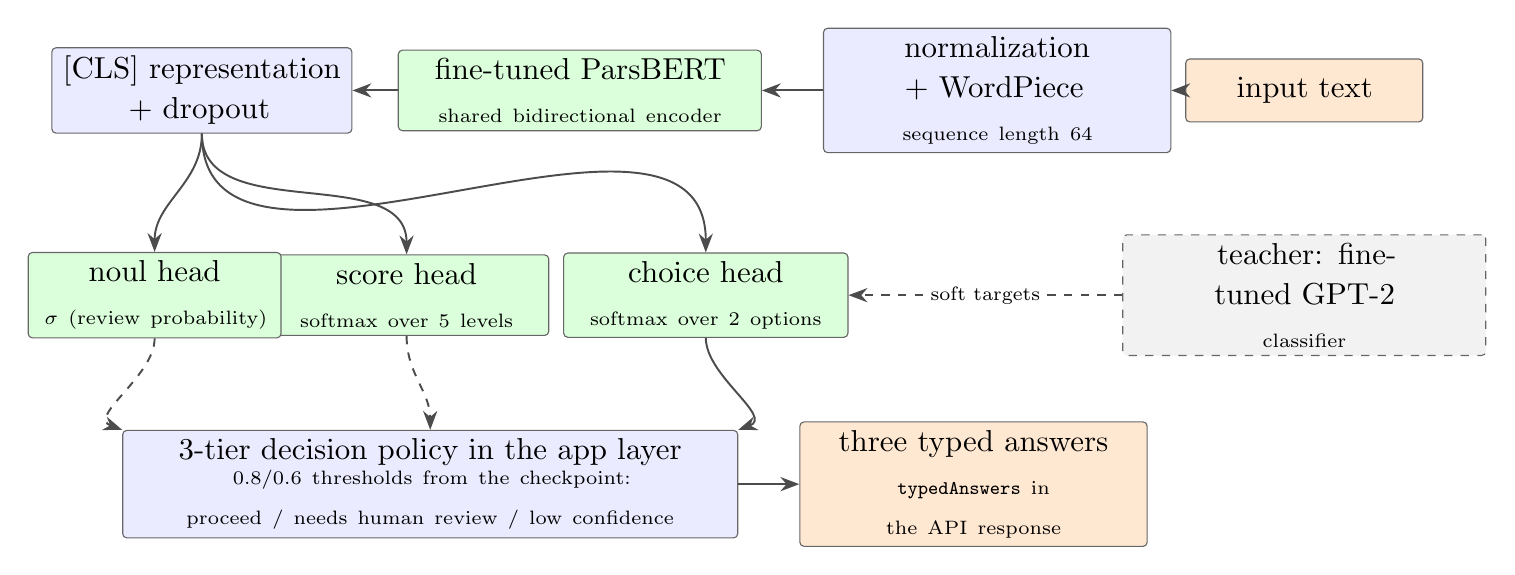
\begin{tikzpicture}
  \node[data, w=2.8cm] (j1) at (0,0) {input text};
  \node[box, w=4.2cm] (j2) at (-3.9,0)
      {normalization + \en{WordPiece}\\[1pt]\scriptsize sequence length \en{64}};
  \node[proc, w=4.4cm] (j3) at (-9.2,0)
      {fine-tuned \en{ParsBERT}\\[1pt]\scriptsize shared bidirectional encoder};
  \node[box, w=3.6cm] (j4) at (-14.0,0)
      {\en{[CLS]} representation\\+ \en{dropout}};
  % three decision heads
  \node[proc, w=3.4cm] (h1) at (-7.6,-2.6)
      {choice head\\[1pt]\scriptsize \en{softmax} over \en{2} options};
  \node[proc, w=3.4cm] (h2) at (-11.4,-2.6)
      {score head\\[1pt]\scriptsize \en{softmax} over \en{5} levels};
  \node[proc, w=3.0cm] (h3) at (-14.6,-2.6)
      {noul head\\[1pt]\scriptsize $\sigma$ (review probability)};
  \draw[arr] (j4.south) to[out=-90,in=90] (h3.north);
  \draw[arr] (j4.south) to[out=-90,in=90] (h2.north);
  \draw[arr] (j4.south) to[out=-90,in=90] (h1.north);
  % distillation teacher
  \node[ext, w=4.4cm] (tch) at (0,-2.6)
      {\en{teacher: fine-tuned GPT-2}\\[1pt]\scriptsize classifier};
  \draw[arrd] (tch.west) -- node[lbl] {soft targets} (h1.east);
  % decision policy
  \node[box, w=7.6cm] (pol) at (-11.1,-5.0)
      {\en{3}-tier decision policy in the app layer\\[1pt]
       \scriptsize \en{0.8}/\en{0.6} thresholds from the checkpoint:\\
       \scriptsize proceed / needs human review / low confidence};
  \draw[arr] (h1.south) to[out=-90,in=20] (pol.north east);
  \draw[arrd] (h2.south) to[out=-90,in=90] (pol.north);
  \draw[arrd] (h3.south) to[out=-90,in=160] (pol.north west);
  \node[data, w=4.2cm] (out) at (-4.2,-5.0)
      {three typed answers\\[1pt]\scriptsize \texttt{typedAnswers} in the \en{API} response};
  \draw[arr] (pol.east) -- (out.west);
  % main flow
  \draw[arr] (j1) -- (j2);
  \draw[arr] (j2) -- (j3);
  \draw[arr] (j3) -- (j4);
\end{tikzpicture}}%
\caption{معماری لایهٔ تصمیم سیستم-یک (\en{JEV}): بدنهٔ مشترک \en{ParsBERT} و
سه سر تصمیم موازی. پیکان نقطه‌چین از معلم \en{GPT-2} فقط در زمان آموزش
(ساخت هدف‌های نرم) برقرار است؛ در زمان سرویس، سه سر خروجی خود را به سیاست
سه‌سطحی در لایهٔ برنامه می‌دهند.}
\label{fig:jev-arch}
\end{figure}

\subsection{هدف‌های نرمِ تقطیرشده از معلم}
چالش اصلی آموزش آن است که مجموعه داده فقط برچسب دودویی دارد، در حالی که
سه سر مدل به هدف‌های احتمالاتی نیاز دارند. راه‌حل، تقطیر دانش از
پروزن‌ترین مدل مستقر در رأی‌گیری ترکیبی است: برای هر نمونه، احتمال معلم
($p_{\text{teacher}}$) از دسته‌بند \en{GPT-2} فاین‌تیون‌شده
(بخش~\ref{sec:tokenizer-improvement})—با دقیقاً همان مسیر سرویس: همان
نرمال‌سازی سطح کاراکتر، همان توکن‌ساز و همان طول توالی ثبت‌شده در
چک‌پوینت معلم—محاسبه و سه هدف نرم ساخته می‌شود:
\begin{itemize}[rightmargin=1em]
  \item \textbf{هدف انتخاب:} ترکیب برچسب واقعی و احتمال معلم،
    $t_{\text{AI}} = \operatorname{clip}(0.8\,y + 0.2\,p_{\text{teacher}},\;
    0.02,\; 0.98)$؛ در نمونه‌های ناسازگار با معلم، هدف عمداً مرزی می‌شود؛
  \item \textbf{هدف امتیاز:} گاوسی گسسته‌شده روی پنج سطح با مرکز
    $4\,t_{\text{AI}}$ و انحراف معیار $\sigma = 0.9$، که یادگیریِ
    «پاسخ میان سطوح» را ممکن می‌کند؛
  \item \textbf{هدف نول:} $1$ تنها هنگامی که خودِ معلم نامطمئن است
    ($0.15 \le p_{\text{teacher}} \le 0.85$)؛ یعنی دقیقاً نمونه‌هایی که
    بازبینی انسانی در آن‌ها ارزش افزوده دارد.
\end{itemize}
تابع هزینه، مجموع وزن‌دار آنتروپی متقاطع نرم روی دو توزیع و آنتروپی متقاطع
دودویی سر نول است:
\begin{equation}
  \mathcal{L} \;=\; \mathcal{L}_{\text{choice}}
  \;+\; 0.5\,\mathcal{L}_{\text{score}}
  \;+\; 0.5\,\mathcal{L}_{\text{noul}}.
\end{equation}

\subsection{سیاست تصمیم و یکپارچه‌سازی در سرویس}
خروجی خام سرها در لایهٔ برنامه به یک \textbf{سیاست سه‌سطحی} تبدیل
می‌شود—همان الگوی توصیه‌شده در راهنمای \en{JEV} مبنی بر اینکه آستانه‌ها و
اقدام نهایی باید در برنامه باشد، نه در مدل: اطمینان
$\max(p^{\text{choice}}) \ge 0.8$ به معنای «ادامه»،
$\max(p^{\text{choice}}) \ge 0.6$ به معنای «نیازمند بازبینی انسانی» و
کمتر از آن به معنای «اطمینان پایین؛ تصمیم خودکار توصیه نمی‌شود» است.
در لایهٔ سرویس، معماری مبتنی بر فیلد \texttt{runtime}
(بخش~\ref{sec:service-arch}) با مقدار تازهٔ
\texttt{\lr{pytorch-jev}} گسترش یافته است. چک‌پوینت تازه، خودکفا است:
پیکربندی کامل بدنهٔ \en{BERT} درون آن ذخیره می‌شود و سرور رمزگذار را بدون
هیچ دسترسی به شبکه بازسازی و وزن‌های فاین‌تیون‌شده (بدنه و سرها) را از
\texttt{\lr{state\_dict}} بار می‌کند. برخلاف طراحی نخست که این مدل را از
ترکیب وزن‌دار کنار می‌گذاشت، اکنون سؤال انتخاب آن در رأی‌گیری وزن‌دار
شرکت می‌کند: احتمال گزینهٔ «تولیدشده توسط هوش مصنوعی» با وزن ثبت‌شده در
\texttt{models.json} در میانگین وزن‌دار ترکیب می‌شود. پاسخ \en{API} نیز
میدان تازهٔ \texttt{\lr{typedAnswers}} را شامل می‌شود و رابط وب، پنل نمایش
سه پاسخ (توزیع انتخاب، متر طیف امتیاز و احتمال بازبینی) را افزوده است.

\subsection{ارزیابی}
معیارهای این مدل به تفکیک نوع سؤال گزارش می‌شوند: دقت/$F_1$ برای پاسخ
انتخاب، خطای مطلق میانگینِ مقدار وزن‌دار برای پاسخ امتیاز، \en{AUC} برای
رتبه‌بندی نیاز به بازبینی، و خطای کالیبراسیون (\en{ECE}) توزیع انتخاب.
آموزش با هدف‌های نرم معلم روی زیرنمونهٔ $6{,}000/1{,}500$ اجرا شده و روی
بخش آزمون به دقت/$F_1$ برابر $0.9893$ رسیده است (ماتریس درهم‌ریختگی
$742/8/8/742$ از $1{,}500$ نمونه)؛ پاسخ امتیاز با خطای مطلق میانگین
$0.0493$ روی طیف $0$ تا $4$ تقریباً بی‌خطاست، توزیع انتخاب با \en{ECE}
برابر $0.0156$ خوب‌کالیبره است و سر نول به \en{AUC} برابر $0.7199$
می‌رسد. چک‌پوینت حاصل—همراه پیکربندی کامل بدنه—جایگزین نسخهٔ پیشین در
سرویس شده است.

\section{سیگنال سرگشتگی مدل زبانی خام: یک بررسی تجربی}
\label{sec:perplexity-signal}
تمام مدل‌های تا اینجا برای تفکیک دو کلاس \textbf{آموزش دیده‌اند}؛ سؤال
مکمل آن است که یک شاخص بدون‌آموزش و مستقل از برچسب‌ها چقدر اطلاعات
دارد. ساده‌ترین چنین شاخصی، سرگشتگی (\en{perplexity}) متن تحت همان مدل
زبانی پیش‌آموزش‌دیدهٔ \en{GPT-2-fa} است: نماییِ میانگین منفی لگاریتم
احتمال توکن‌های متن، یعنی «میزان تعجب» مدل از متن. انتظار متداول آن
است که متن تولیدشده توسط هوش مصنوعی — که خود خروجی یک مدل زبانی است —
تحت یک مدل مرجع قابل‌پیش‌بینی‌تر (سرگشتگی کمتر) از متن انسان باشد.

در سرویس این شاخص کم‌هزینه است: مدل از پیش بار شده و محاسبه تنها یک
گذر رو به جلو با همان مسیر سرویس (نرمال‌سازی، توکن‌ساز و برش کاراکتری
مشترک) و پنجرهٔ $64$ توکن است. سرگشتگی به‌عنوان جزئیات تحلیلی تازه—در
کنار آنتروپی، تنوع جمله، تکرار و انسجام—در پاسخ \en{API} و رابط وب
نمایش داده می‌شود و عمداً هیچ وزنی در ترکیب وزن‌دار ندارد.

ارزیابی روی $1{,}500$ متن بخش آزمون، انتظار متداول را رد می‌کند:
\en{AUC} سرگشتگی به‌عنوان نمرهٔ تشخیص فقط $0.3387$ است، یعنی جهت
سیگنال \textbf{وارونه} است (با برگرداندن جهت: $0.6613$). توزیع دو
کلاس به‌شدت هم‌پوشان است—میانهٔ سرگشتگی متن‌های هوش‌مصنوعی $50.6$ در
برابر $30.7$ برای متن‌های انسانی—و بهترین آستانهٔ \en{Youden} تنها به
دقت $0.526$ می‌رسد. تفسیر محتمل، همان ناهم‌خوانی مدل مرجع است: متن‌های
تولیدی $70$ مدل بسیار قوی‌تر از \en{GPT-2} با $124$ میلیون پارامتر، از
زاویهٔ این مدل کوچک «غافلگیرکننده‌تر» از وبلاگ‌های انسانی‌اند. نتیجهٔ
عملی: سرگشتگی مدل مرجع کوچک در این مجموعه هم به‌تنهایی تشخیص‌دهندهٔ
ضعیفی است و هم جهتی برخلاف شهود دارد؛ پس صرفاً به‌عنوان شاخص نمایشی
نگه داشته شده و ورودش به ترکیب، منوط به بررسی با مدل مرجع قوی‌تر یا
رویکردهای اغتشاش‌محور است.

% -----------------------------------------------------------------------------
% -----------------------------------------------------------------------------
\chapter{تنظیم هایپرپارامتر و اعتبارسنجی متقابل}
\label{sec:hpo}
% -----------------------------------------------------------------------------

یکی از یافته‌های اصلی این گزارش آن است که \textbf{هیچ‌یک} از مدل‌های
کلاسیک در نسخهٔ نخست، هیچ جست‌وجوی هایپرپارامتری را پشت سر نگذاشته بودند؛
تمام آن‌ها با مقادیر پیش‌فرض کتابخانهٔ \en{scikit-learn} آموزش دیده بودند.
خط‌لولهٔ اصلاح‌شده برای هر مدل کلاسیک، جست‌وجوی هایپرپارامتر را با
اعتبارسنجی متقابل $k$-تاخورده (\en{k-fold cross-validation}) \textbf{تنها
روی مجموعهٔ آموزش} انجام می‌دهد (جدول~\ref{tab:hpo}) و مدل نهایی را با
بهترین هایپرپارامترها روی مجموعهٔ آموزش+اعتبارسنجی ترکیبی بازآموزش
می‌دهد، پیش از ارزیابی نهایی و یک‌باره روی مجموعهٔ آزمون.

\begin{table}[H]
\centering
\caption{فضای جست‌وجوی هایپرپارامتر برای هر مدل کلاسیک}
\label{tab:hpo}
\begin{tabular}{lll}
\toprule
\textbf{مدل} & \textbf{روش جست‌وجو} & \textbf{هایپرپارامترهای تنظیم‌شده} \\
\midrule
\en{SVM} & \en{RandomizedSearchCV} ($k{=}5$) & $C$، تابع زیان، وزن کلاس \\
رگرسیون لجستیک & \en{RandomizedSearchCV} ($k{=}5$) & $C$، حل‌کننده، وزن کلاس \\
بیز ساده & \en{GridSearchCV} ($k{=}5$) & $\alpha$ \\
جنگل تصادفی & \en{RandomizedSearchCV} ($k{=}3$) & تعداد درخت، عمق، برگ کمینه \\
گرادیان بوستینگ & \en{RandomizedSearchCV} ($k{=}3$) & تعداد درخت، عمق، نرخ یادگیری \\
\bottomrule
\end{tabular}
\end{table}

معیار بهینه‌سازی در تمام جست‌وجوها امتیاز $F_1$ است (نه دقت خام)، زیرا در
یک مسئلهٔ متوازن دودویی، $F_1$ حساسیت بهتری به تعادل میان دقت مثبت
(\en{precision}) و بازیابی (\en{recall}) نشان می‌دهد.

% -----------------------------------------------------------------------------
\chapter{معیارهای ارزیابی}
% -----------------------------------------------------------------------------

برای هر مدل، ماتریس درهم‌ریختگی (\en{confusion matrix}) با چهار عنصر
\en{TP} (مثبت درست)، \en{TN} (منفی درست)، \en{FP} (مثبت کاذب) و
\en{FN} (منفی کاذب) محاسبه و معیارهای زیر از آن استخراج می‌شود:
\begin{align}
  \text{دقت (\en{Accuracy})} &= \frac{TP+TN}{TP+TN+FP+FN} \\
  \text{دقت مثبت (\en{Precision})} &= \frac{TP}{TP+FP} \\
  \text{بازیابی (\en{Recall})} &= \frac{TP}{TP+FN} \\
  F_1 &= 2\cdot\frac{\text{Precision}\times\text{Recall}}{\text{Precision}+\text{Recall}}
\end{align}
در این کاربرد، \en{FP} (طبقه‌بندی نادرست متن انسانی به‌عنوان هوش مصنوعی)
معمولاً هزینهٔ اجتماعی بالاتری دارد (مثلاً اتهام نادرست تقلب به یک نویسندهٔ
انسانی)؛ به همین دلیل $\text{Precision}$ و $F_1$ در کنار دقت خام، معیارهای
اصلی گزارش‌دهی این پروژه‌اند.

% -----------------------------------------------------------------------------
\chapter{زیرساخت پیاده‌سازی}
% -----------------------------------------------------------------------------

\section{معماری سرویس}
\label{sec:service-arch}
بک‌اند با چارچوب \en{FastAPI} (پایتون) پیاده‌سازی شده و از یک الگوی
\textbf{اعزام عمومی بر اساس نوع اجرا} (\en{runtime dispatch}) استفاده
می‌کند: هر مدل در \texttt{models.json} یک فیلد \texttt{runtime} دارد
(\texttt{sklearn-tfidf}، \texttt{pytorch-lstm}، \texttt{pytorch-gpt2} یا
\texttt{pytorch-jev}) و منطق بارگذاری/استنتاج بر اساس همین فیلد انتخاب
می‌شود. این طراحی امکان
می‌دهد مدل‌های جدید—صرف‌نظر از خانوادهٔ الگوریتمی—بدون تغییر در نقاط پایانی
(\en{endpoints}) \en{API} افزوده شوند. رابط کاربری وب (\en{Next.js} +
\en{React}) به‌طور کامل بر اساس دادهٔ بازگشتی از \texttt{/models} ساخته
می‌شود؛ مدل‌ها بر اساس نوع (یادگیری ماشین کلاسیک در برابر یادگیری عمیق)
دسته‌بندی و یک نمودار مقایسهٔ تعاملی میان تمام مدل‌ها نمایش داده می‌شود.

شکل~\ref{fig:deployment} نمای استقرار اجزا و مسیرهای ارتباطی را نشان می‌دهد.
دو نکتهٔ طراحی در این نما دیده می‌شود: نخست، کلید \en{API} سرویس آنلاین
هرگز در سرور ذخیره نمی‌شود و فقط همراه همان درخواست از پروکسی \en{Next.js}
عبور می‌کند؛ دوم، سرور پایتون همهٔ آرتیفکت‌ها را یک‌بار در زمان راه‌اندازی
(\texttt{init()}) بار می‌کند تا هیچ درخواستی هزینهٔ بارگذاری سرد
(\en{cold load}) نپردازد. نقطهٔ پایانی \en{GET /models} نیز فیلدهای
پیاده‌سازی (\texttt{runtime}، \texttt{filename}، \texttt{vectorizer}) را
پیش از ارسال حذف می‌کند و «مدل ترکیبی» را — که مدلی مستقل نیست و در هر
درخواست همهٔ مدل‌ها را اجرا می‌کند — به‌عنوان مدخل نخست و انتخاب پیش‌فرض
برمی‌گرداند.

\begin{figure}[H]
\centering
\resizebox{0.95\textwidth}{!}{%
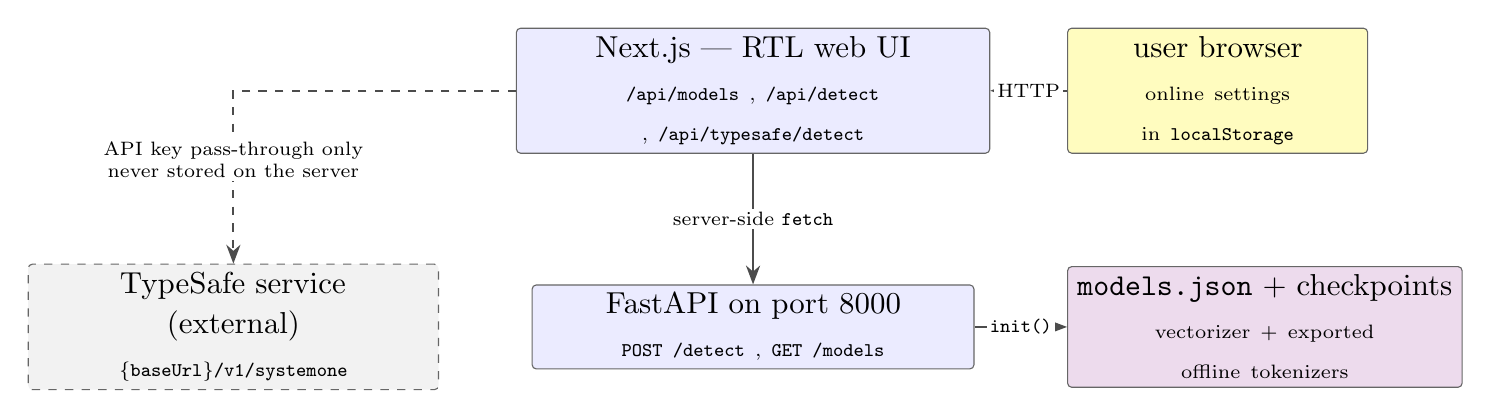
\begin{tikzpicture}
  \node[usr, w=3.6cm] (br) at (0,0)
      {user browser\\[1pt]\scriptsize online settings in \texttt{localStorage}};
  \node[box, w=5.8cm] (nx) at (-5.9,0)
      {\en{Next.js} — RTL web UI\\[1pt]\scriptsize
       \texttt{/api/models} , \texttt{/api/detect} , \texttt{/api/typesafe/detect}};
  \node[box, w=5.4cm] (api) at (-5.9,-3.0)
      {\en{FastAPI} on port \en{8000}\\[1pt]\scriptsize \texttt{POST /detect} , \texttt{GET /models}};
  \node[art, w=4.8cm] (art) at (0.6,-3.0)
      {\texttt{models.json} + checkpoints\\[1pt]\scriptsize vectorizer + exported offline tokenizers};
  \node[ext, w=5.0cm] (ts) at (-12.5,-3.0)
      {\en{TypeSafe} service\\(external)\\[1pt]\scriptsize \texttt{\{baseUrl\}/v1/systemone}};
  \draw[arr] (br) -- node[lbl] {\en{HTTP}} (nx);
  \draw[arr] (nx.south) -- node[lbl] {server-side \texttt{fetch}} (api.north);
  \draw[arr] (api.east) -- node[lbl] {\texttt{init()}} (art.west);
  \draw[arrd] (nx.west) -| node[lbl, pos=0.7] {\en{API} key pass-through only\\never stored on the server} (ts.north);
\end{tikzpicture}}%
\caption{نمای استقرار سامانه. مرورگر فقط با رابط وب \en{Next.js} حرف می‌زند؛
درخواست‌های محلی از پروکسی سمت سرور به \en{FastAPI} و درخواست آنلاین به
سرویس بیرونی \en{TypeSafe} می‌رود. پیکان‌ها جهت فراخوانی را نشان می‌دهند و
پاسخ در همان مسیر برمی‌گردد.}
\label{fig:deployment}
\end{figure}

جدول~\ref{tab:runtimes} قرارداد اعزام زمان اجرا را خلاصه می‌کند: هر مقدار
\texttt{runtime} در \texttt{models.json} به یک جفت تابع بارگذار/پیش‌بین در
بستهٔ \texttt{aitextd} نگاشت می‌شود (\texttt{loaders.py} و
\texttt{predictors.py}) و مسیر پیش‌پردازش متناسب با آن خانواده را تعیین
می‌کند. ناهم‌خوانی آموزش/سرویس (بخش‌های~\ref{sec:tokenizer-improvement}
و~\ref{sec:style-features}) دقیقاً در همین قرارداد کنترل می‌شود: همان
توکن‌ساز صادرشدهٔ آفلاین، همان نرمال‌سازی و همان فرمول ویژگی‌های سبکی که در
آموزش به‌کار رفته، در سرویس هم به‌کار می‌رود.

\begin{table}[H]
\centering
\caption{رجیستری زمان اجرا: نگاشت فیلد \texttt{runtime} به بارگذار، آرتیفکت و مسیر پیش‌پردازش}
\label{tab:runtimes}
\begin{tabular}{p{3.7cm}p{2.3cm}p{4.7cm}p{3.3cm}}
\toprule
\textbf{\texttt{runtime}} & \textbf{مدل‌ها} & \textbf{آرتیفکت بارگذاری‌شده} & \textbf{مسیر پیش‌پردازش} \\
\midrule
\texttt{sklearn-tfidf} & ۵ مدل کلاسیک &
چک‌پوینت \en{joblib} هر مدل به‌همراه بردارساز مشترک \mbox{\en{TF-IDF}} &
خط‌لولهٔ کامل \en{shekar} (ریشه‌یابی + توکن‌سازی) \\
\texttt{pytorch-lstm} & \en{BiLSTM} &
چک‌پوینت شامل وزن‌ها، واژگان و پیکربندی &
خط‌لولهٔ کامل \en{shekar} \\
\texttt{pytorch-gpt2} & \en{GPT-2} &
سر طبقه‌بندی + بدنهٔ پیش‌آموزش‌دیده + توکن‌ساز صادرشدهٔ آفلاین &
فقط نرمال‌سازی سطح کاراکتر \\
\texttt{pytorch-parsbert} & \en{ParsBERT} &
چک‌پوینت خودکفا (پیکربندی بدنه درون چک‌پوینت) + توکن‌ساز &
فقط نرمال‌سازی سطح کاراکتر \\
\texttt{pytorch-jev} & لایهٔ تصمیم \en{JEV} &
چک‌پوینت بدنه + سه سر تصمیم + آستانه‌های سیاست &
فقط نرمال‌سازی سطح کاراکتر \\
\bottomrule
\end{tabular}
\end{table}

\section{جریان پردازش یک درخواست تشخیص}
\label{sec:inference-flow}
شکل~\ref{fig:inference-flow} مسیر یک درخواست از لحظهٔ ورود تا ساخت پاسخ را
نشان می‌دهد. نکتهٔ کلیدی طراحی، واحد بودن مسیر آماده‌سازی برای همهٔ
مدل‌هاست: پیش‌پردازش متناسب با مدل انتخابی انجام می‌شود، اما چهار ویژگی
سبک‌شناسی بخش~\ref{sec:style-features} و سرگشتگی بخش~\ref{sec:perplexity-signal}
یک‌بار و مستقل از مدل محاسبه می‌شوند و هم به‌عنوان ورودی/جزئیات تحلیلی و هم
برای نمایش در پاسخ به‌کار می‌روند. در حالت ترکیبی، هر مدل با وزن
\texttt{ensembleWeight} خود در رأی‌گیری شرکت می‌کند — در پیکربندی کنونی
\en{GPT-2} وزن $3$، لایهٔ \en{JEV} وزن $0.6$ و بقیه وزن $1$ دارند؛ وزن صفر
به معنای خروج اختیاری از رأی است — و پاسخ نهایی، میانگین وزن‌دار احتمال
هوش‌مصنوعی‌بودن همهٔ مدل‌هاست.

\begin{figure}[H]
\centering
\resizebox{0.98\textwidth}{!}{%
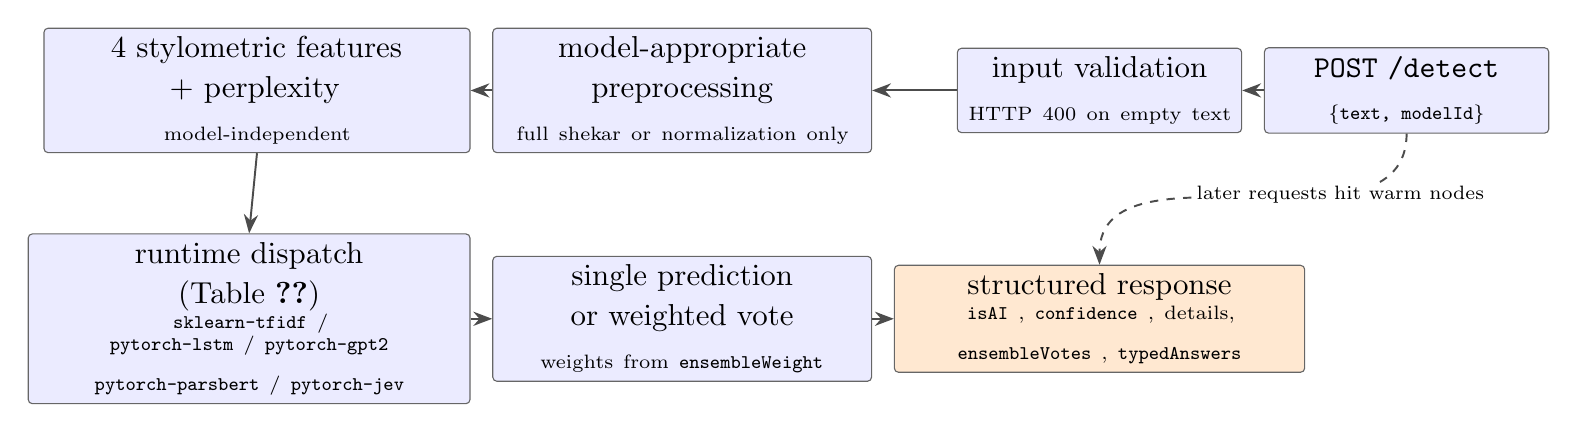
\begin{tikzpicture}
  \node[box, w=3.4cm] (req) at (0,0)
      {\texttt{POST /detect}\\[1pt]\scriptsize \texttt{\{text, modelId\}}};
  \node[box, w=3.4cm] (val) at (-3.9,0)
      {input validation\\[1pt]\scriptsize \en{HTTP} \en{400} on empty text};
  \node[box, w=4.6cm] (prep) at (-9.2,0)
      {model-appropriate preprocessing\\[1pt]\scriptsize full \en{shekar} or normalization only};
  \node[box, w=5.2cm] (style) at (-14.6,0)
      {\en{4} stylometric features\\+ perplexity\\[1pt]\scriptsize model-independent};
  \node[box, w=5.4cm] (disp) at (-14.7,-2.9)
      {runtime dispatch\\(Table~\ref{tab:runtimes})\\[1pt]\scriptsize
       \texttt{sklearn-tfidf} / \texttt{pytorch-lstm} / \texttt{pytorch-gpt2}\\
       \texttt{pytorch-parsbert} / \texttt{pytorch-jev}};
  \node[box, w=4.6cm] (pred) at (-9.2,-2.9)
      {single prediction or weighted vote\\[1pt]\scriptsize weights from \texttt{ensembleWeight}};
  \node[data, w=5.0cm] (resp) at (-3.9,-2.9)
      {structured response\\[1pt]\scriptsize \texttt{isAI} , \texttt{confidence} , details,\\
       \texttt{ensembleVotes} , \texttt{typedAnswers}};
  \draw[arr] (req) -- (val);
  \draw[arr] (val) -- (prep);
  \draw[arr] (prep) -- (style);
  \draw[arr] (style.south) -- (disp.north);
  \draw[arr] (disp.east) -- (pred.west);
  \draw[arr] (pred.east) -- (resp.west);
  \draw[arrd] (req.south) to[out=-90,in=90] node[lbl, pos=0.3] {later requests hit warm nodes} (resp.north);
\end{tikzpicture}}%
\caption{جریان پردازش یک درخواست تشخیص در بک‌اند. تمام مدل‌ها و توکن‌سازها
در زمان راه‌اندازی سرور بار و گرم می‌شوند؛ درخواست هر کاربر صرفاً یک گذر
استنتاج است.}
\label{fig:inference-flow}
\end{figure}

\section{ساختار پروژه}
\label{sec:repo-layout}
ساختار پوشه‌های مخزن، نقشهٔ کلی همهٔ فصل‌های این گزارش است:
\begin{LTRverb}
\begin{verbatim}
AITextDetection/
|-- server.py             thin launcher: python server.py
|-- models.json           registry of the 9 models (runtime, weights)
|-- pyproject.toml        deps + tooling (uv, ruff, pytest)
|-- aitextd/              shared package: serving + training
|   |-- paths.py          all filesystem paths (data/, models/)
|   |-- text.py           Persian preprocessing
|   |-- features.py       stylometric features
|   |-- architectures.py  torch model architectures
|   |-- loaders.py        per-runtime model loading
|   |-- predictors.py     per-runtime prediction
|   |-- jev.py            JEV typed answers + policy
|   |-- store.py          registry + detection orchestration
|   `-- api.py            FastAPI application
|-- data/                 datasets (raw CSVs + processed)
|-- models/               artifacts + exported tokenizers
|-- training/             local training scripts (root)
|-- notebooks/
|   `-- colab_training.ipynb   unified GPU retraining
|-- tests/                pytest: -m not-slow / -m slow golden
|-- web-app/              Next.js front end (RTL, Persian)
`-- report/               this report (XeLaTeX source)
\end{verbatim}
\end{LTRverb}
پنج نکته در این چیدمان عمدی است: (۱) همهٔ مسیرهای فایل‌سیستم در یک نقطه
متمرکز شده‌اند (\texttt{\lr{aitextd/paths.py}})؛ مجموعه‌داده‌ها در
\texttt{\lr{data/}} و آرتیفکت‌های آموزش‌دیده در \texttt{\lr{models/}}
نگهداری می‌شوند و ریشهٔ پروژه با متغیر محیطی
\texttt{\lr{AITEXTD\_ROOT}} نیز قابل جابه‌جایی است؛ (۲) توکن‌سازها به‌صورت
پوشه‌های صادرشده کنار چک‌پوینت‌ها در \texttt{\lr{models/}} نگهداری می‌شوند
تا سرویس هیچ وابستگی شبکه‌ای به \en{Hugging Face Hub} نداشته باشد
(بخش~\ref{sec:tokenizer-improvement})؛ (۳) خط‌لولهٔ بازتولید محلی در پوشهٔ
\texttt{\lr{training/}} و نوت‌بوک یکپارچهٔ \en{GPU} در
\texttt{\lr{notebooks/colab\_training.ipynb}} است (پیوست~\ref{app:runbook})؛
(۴) منطق مشترک آموزش/سرویس — پیش‌پردازش، ویژگی‌ها، معماری‌ها و شمای
\en{JEV} — فقط یک‌بار در بستهٔ \texttt{\lr{aitextd/}} پیاده‌سازی شده و هم
سرور و هم همهٔ مسیرهای آموزش همان کد را وارد می‌کنند؛ در نتیجه ناهم‌خوانی
آموزش/سرویس از نظر ساختاری ناممکن است؛ و (۵) رابط وب از بک‌اند جداست و
فقط از طریق پروکسی‌های سمت سرور با آن حرف می‌زند
(شکل~\ref{fig:deployment}).

\section{تحلیل آنلاین با مدل \en{System One} سرویس \en{TypeSafe}}
\label{sec:online-systemone}
علاوه بر مدل‌های محلی، رابط وب حالتی را افزوده است که همان متن را به مدل
\en{System One} سرویس \en{TypeSafe}—مدل تجاری تصمیم سریع که لایهٔ محلی
\en{JEV} به سبک آن ساخته شده بود—می‌سپارد. برای آنکه مقایسه معنادار بماند،
سه سؤال نوع‌بندی‌شدهٔ ارسالی عیناً قرینهٔ سؤالات محلی است: سؤال انتخاب با دو
گزینهٔ \texttt{\lr{human\_written}}/\texttt{\lr{ai\_generated}}، سؤال امتیاز
پنج‌سطحی «ماشین‌مانندبودن سبک نوشتار» با توصیف‌های مستقل و موقعیت‌مند برای هر
سطح، و سؤال نولِ نیاز به بازبینی انسانی. سیاست سه‌سطحی تصمیم نیز همان
آستانه‌های چک‌پوینت محلی ($0.8$/$0.6$) را روی $\max(p^{\text{choice}})$ اعمال
می‌کند؛ «اطمینان انتخاب» خود مدل—تمرکز توزیع احتمال، نه اندازهٔ آن—جداگانه در
پاسخ \en{API} برگردانده و در رابط نمایش داده می‌شود.

از آنجا که مرورگر نمی‌تواند سرویس خارجی را مستقیم فراخوانی کند (محدودیت
\en{CORS})، درخواست از مسیری سمت سرور در \en{Next.js}
(\texttt{\lr{/api/typesafe/detect}}) عبور می‌کند: این مسیر بدنه را به
\texttt{\lr{\{baseUrl\}/v1/systemone}} با سرآیند
\texttt{\lr{Authorization: Bearer}} ارسال می‌کند، خطاهای شناخته‌شدهٔ سرویس
($401/422/429/529$) و زمان انتظار را به پیام‌های فارسی نگاشت می‌کند و پاسخ را
به همان ساختار نتایج تشخیص محلی برمی‌گرداند تا اجزای نمایش بازبه‌کار شوند.
تنظیمات اتصال (کلید \en{API}، آدرس پایه و نام مدل) توسط کاربر در پنلی در
صفحهٔ اصلی وارد و صرفاً در \texttt{\lr{localStorage}} مرورگر ذخیره می‌شود؛
سرور هیچ‌گاه کلید را ذخیره نمی‌کند و تنها همراه همان درخواست به مقصد ارسال
می‌گردد. آدرس پایه هم به شکل مبدأ خام پذیرفته می‌شود و هم آدرس کامل نقطهٔ
پایان (حاوی پسوند \texttt{\lr{/v1/systemone}})؛ نام مدل نیز دلخواه است
(\texttt{\lr{jev-latest}} پیش‌فرض). برای هم‌گام‌ماندن تنظیمات میان زبانه‌ها،
خواندن و نوشتن تنظیمات از طریق \texttt{\lr{useSyncExternalStore}} انجام
می‌شود.

سه حالت تحلیل در رابط وب ارائه شده است: «محلی»، «آنلاین» و «مقایسه هر دو».
در حالت سوم هر دو موتور به‌طور موازی روی همان متن اجرا می‌شوند
(\texttt{\lr{Promise.allSettled}}) تا خطای یک سمت، نتیجهٔ سمت دیگر را پنهان
نکند. کارت مقایسه، دو موتور را به‌صورت ستون‌های کنار هم ردیف می‌کند—نتیجه،
احتمال هوش‌مصنوعی‌بودن، اطمینان، مقدار امتیاز ماشین‌مانندبودن و احتمال نیاز
به بازبینی—و نشانِ «نتیجه یکسان» یا «مغایرت در نتیجه» نمایش می‌دهد. برای
هم‌ترازی پاسخ‌های نوع‌بندی‌شده، سمت محلی در این حالت به‌طور پیش‌فرض روی مدل
\texttt{\lr{jev\_system\_one}} قرار می‌گیرد، نه رأی ترکیبی؛ چون میانگین وزن‌دار
پاسخ نوع‌بندی‌شده ندارد و ستون‌های آن در ماتریس مقایسه خالی می‌ماند.
شکل~\ref{fig:online-flow} این دو مسیر موازی را نشان می‌دهد: هر دو موتور
هم‌زمان و مستقل اجرا می‌شوند و شکست یکی، دیگری را از کار نمی‌اندازد.

\begin{figure}[H]
\centering
\resizebox{0.95\textwidth}{!}{%
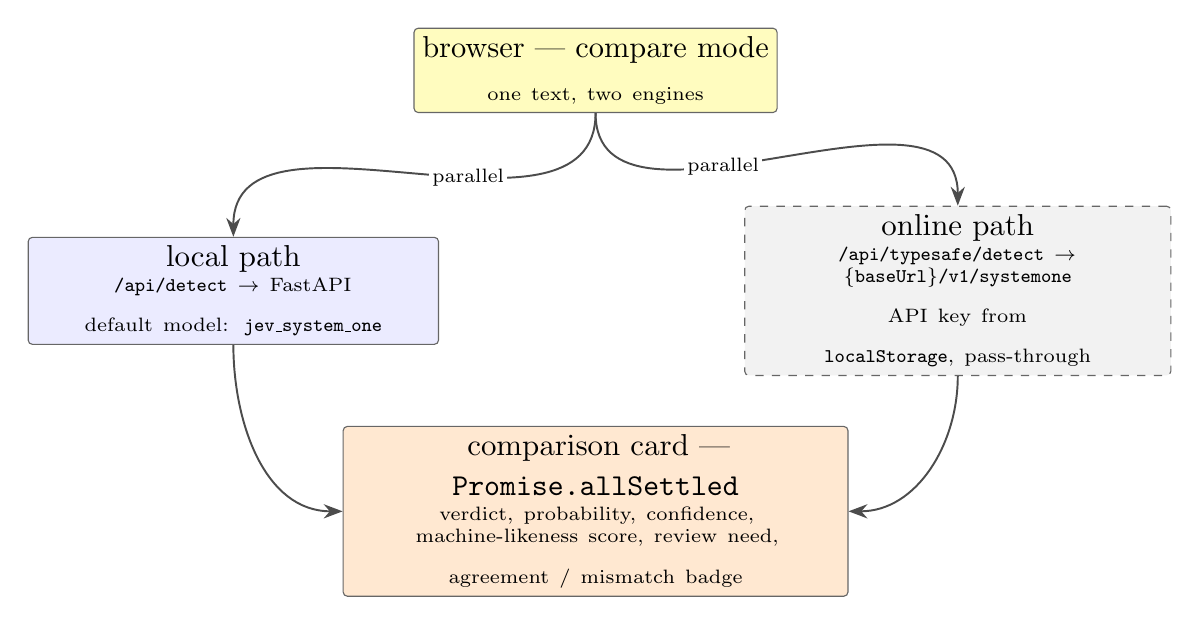
\begin{tikzpicture}
  \node[usr, w=4.4cm] (br) at (-6.0,0)
      {browser — compare mode\\[1pt]\scriptsize one text, two engines};
  \node[box, w=5.0cm] (loc) at (-10.6,-2.8)
      {local path\\[1pt]\scriptsize \texttt{/api/detect} $\to$ \en{FastAPI}\\
       \scriptsize default model: \texttt{jev\_system\_one}};
  \node[ext, w=5.2cm] (onl) at (-1.4,-2.8)
      {online path\\[1pt]\scriptsize \texttt{/api/typesafe/detect} $\to$ \texttt{\{baseUrl\}/v1/systemone}\\
       \scriptsize \en{API} key from \texttt{localStorage}, pass-through};
  \node[data, w=6.2cm] (cmp) at (-6.0,-5.6)
      {comparison card — \texttt{Promise.allSettled}\\[1pt]\scriptsize
       verdict, probability, confidence, machine-likeness score, review need,\\
       \scriptsize agreement / mismatch badge};
  \draw[arr] (br.south) to[out=-90,in=90] node[lbl, pos=0.4] {parallel} (loc.north);
  \draw[arr] (br.south) to[out=-90,in=90] node[lbl, pos=0.4] {parallel} (onl.north);
  \draw[arr] (loc.south) to[out=-90,in=180] (cmp.west);
  \draw[arr] (onl.south) to[out=-90,in=0] (cmp.east);
\end{tikzpicture}}%
\caption{حالت مقایسهٔ آنلاین/محلی. دو درخواست مستقل و موازی ارسال می‌شوند و
\texttt{\lr{Promise.allSettled}} تضمین می‌کند خطای یک مسیر، نتیجهٔ مسیر دیگر
را پنهان نکند.}
\label{fig:online-flow}
\end{figure}

در اجرای واقعی با یک نقطهٔ پایان سازگار با \en{TypeSafe}، هر دو موتور روی یک
متن آزمایشیِ تولیدشده توسط هوش مصنوعی هم‌نظر بودند (هر دو $99\%$) و امتیاز
ماشین‌مانندبودن آنلاین ($3.75$ از $4$) به مقدار محلی ($3.54$) نزدیک بود؛
تنها تفاوت محسوس، احتمال نیاز به بازبینی بود ($70\%$ در برابر $0\%$). این
حالت مکمل مدل‌های محلی است نه جایگزین آن‌ها: زبان اصلی آموزش \en{Jev}
انگلیسی است و مانند مدل‌های محلی، دقت آن روی متن فارسی محدودیت دارد.

\section{محدودیت‌های سخت‌افزار محلی در برابر \en{Google Colab}}
جدول~\ref{tab:infra} تفاوت محیط آموزش نسخهٔ نخست (محلی) و نسخهٔ دوم
(\en{Colab}) را خلاصه می‌کند.

\begin{table}[H]
\centering
\caption{مقایسهٔ محیط آموزش}
\label{tab:infra}
\begin{tabular}{lll}
\toprule
\textbf{ویژگی} & \textbf{محیط محلی} & \textbf{\en{Google Colab}} \\
\midrule
پردازنده & ۱۲ هسته (فقط \en{CPU}) & \en{GPU} (معمولاً \en{T4}) \\
حافظهٔ آزاد دیسک & $\approx 9$--$10$ گیگابایت & به‌مراتب بیشتر \\
فاین‌تیون \en{GPT-2} & زیرنمونه، ۴ بلوک، ۶۴ توکن & کل داده، ۱۲ بلوک، ۱۲۸ توکن \\
جست‌وجوی هایپرپارامتر & انجام نشد & \en{RandomizedSearchCV}/\en{GridSearchCV} \\
\bottomrule
\end{tabular}
\end{table}

این محدودیت‌های سخت‌افزاری علت اصلی طراحی خط‌لولهٔ دوم به‌عنوان نوت‌بوک
یکپارچهٔ \en{Colab} (\texttt{notebooks/colab\_training.ipynb}) به‌جای اجرای
مستقیم روی سرور محلی است.

% -----------------------------------------------------------------------------
\chapter{نتایج و تحلیل خطا}
% -----------------------------------------------------------------------------

\section{نتایج نسخهٔ نخست (محلی)}
\label{sec:results-v1}
جدول~\ref{tab:results-v1} معیارهای اندازه‌گیری‌شدهٔ هفت مدل نسخهٔ نخست را
روی مجموعهٔ آزمون مربوط به هرکدام نشان می‌دهد (این معیارها همان مقادیر
واقعی ثبت‌شده در \texttt{models.json} در زمان تدوین این گزارش‌اند).

\begin{table}[H]
\centering
\caption{معیارهای مدل‌های نسخهٔ نخست (محلی، بدون تنظیم هایپرپارامتر)}
\label{tab:results-v1}
\begin{tabular}{lrrrrr}
\toprule
\textbf{مدل} & \textbf{نوع} & \textbf{دقت} & \textbf{دقت مثبت} & \textbf{بازیابی} & \textbf{$F_1$} \\
\midrule
\en{SVM} (\en{LinearSVC}) & ی.ماشین & $0.9906$ & $0.9971$ & $0.9840$ & $0.9905$ \\
رگرسیون لجستیک & ی.ماشین & $0.9434$ & $0.9916$ & $0.8943$ & $0.9404$ \\
بیز ساده & ی.ماشین & $0.9597$ & $0.9277$ & $0.9972$ & $0.9612$ \\
جنگل تصادفی & ی.ماشین & $0.9685$ & $0.9700$ & $0.9668$ & $0.9684$ \\
گرادیان بوستینگ & ی.ماشین & $0.9334$ & $0.9755$ & $0.8890$ & $0.9303$ \\
\en{BiLSTM} & ی.عمیق & $0.9787$ & $0.9837$ & $0.9734$ & $0.9786$ \\
\en{GPT-2} فاین‌تیون‌شده & ی.عمیق & $0.9807$ & $0.9852$ & $0.9760$ & $0.9806$ \\
\bottomrule
\end{tabular}
\end{table}

\section{چرا مدل‌ها روی متن واقعی اشتباه می‌کردند؟}
\label{sec:v1-error-causes}
با وجود ارقام بالای جدول~\ref{tab:results-v1}، آزمایش دستی مدل‌ها با
متن‌های واقعی (خارج از دو منبع دادهٔ آموزشی) نشان داد که تمام مدل‌ها به‌جز
\en{GPT-2} خطاهای محسوسی مرتکب می‌شوند. این شکاف میان معیار گزارش‌شده و
عملکرد واقعی، نه یک تناقض، بلکه نشانهٔ کلاسیک \textbf{بیش‌برازش به توزیع
دادهٔ آموزش} است. علل مشخص‌شده به شرح زیرند:
\begin{enumerate}[rightmargin=1em]
  \item \textbf{عدم تنظیم هایپرپارامتر} (بخش~\ref{sec:hpo}): تمام مدل‌های
    کلاسیک با مقادیر پیش‌فرض آموزش دیده بودند؛ به‌ویژه نبود تنظیم صریح
    برای وزن‌دهی تنظیم (\en{regularization strength}) در \en{SVM}/رگرسیون
    لجستیک و نبود محدودیت عمق در جنگل تصادفی.
  \item \textbf{فضای ویژگی سه‌گرم‌محور بدون سقف} (بخش~\ref{sec:tfidf-problem}):
    $9.4$ میلیون ویژگی کم‌رخداد، حفظ عبارات دقیق آموزش را به‌جای تعمیم
    تسهیل می‌کرد.
  \item \textbf{نشت ظریف داده در انتخاب مدل} (بخش~\ref{sec:split}): انتخاب
    بهترین دوره با نگاه به مجموعهٔ آزمون.
  \item \textbf{پیش‌پردازش ناسازگار با مدل} (بخش‌های~\ref{sec:gpt2-preprocess}
    و~\ref{sec:tokenizer-improvement}).
\end{enumerate}

\section{اصلاحات اعمال‌شده در نسخهٔ دوم}
هر چهار علت بالا در خط‌لولهٔ \en{Colab} به‌طور مستقیم برطرف شده است:
جست‌وجوی واقعی هایپرپارامتر با اعتبارسنجی متقاطع، فضای ویژگی
$(1,3)$-گرمی با سقف و انتخاب $\chi^2$، تفکیک سه‌گانهٔ
آموزش/اعتبارسنجی/آزمون، و توکن‌ساز سریعِ هم‌راستا با پیش‌آموزش.
(جزئیات در فصل‌های~\ref{sec:hpo} تا~\ref{sec:tokenizer-improvement}.)

\section{نتایج نسخهٔ دوم (\en{Colab}, واقعی)}
\label{sec:results-v1-vs-v2}
جدول~\ref{tab:results-v2} معیارهای مدل‌های بازآموزش‌شده را نشان می‌دهد.

\begin{table}[H]
\centering
\caption{معیارهای مدل‌ها پس از بازآموزی نسخهٔ دوم (\en{Colab})}
\label{tab:results-v2}
\begin{tabular}{lrrrr}
\toprule
\textbf{مدل} & \textbf{دقت} & \textbf{دقت مثبت} & \textbf{بازیابی} & \textbf{$F_1$} \\
\midrule
\en{SVM} & $0.9950$ & $0.9948$ & $0.9953$ & $0.9950$ \\
رگرسیون لجستیک & $0.9955$ & $0.9971$ & $0.9938$ & $0.9955$ \\
بیز ساده & $0.9808$ & $0.9889$ & $0.9725$ & $0.9806$ \\
جنگل تصادفی & $0.9836$ & $0.9880$ & $0.9791$ & $0.9836$ \\
گرادیان بوستینگ & $0.9919$ & $0.9976$ & $0.9862$ & $0.9919$ \\
\en{BiLSTM} & $0.9832$ & $0.9894$ & $0.9768$ & $0.9831$ \\
\en{GPT-2} فاین‌تیون‌شده & $0.9969$ & $0.9962$ & $0.9976$ & $0.9969$ \\
\en{ParsBERT} فاین‌تیون‌شده & $0.9983$ & $0.9981$ & $0.9986$ & $0.9983$ \\
\bottomrule
\end{tabular}
\end{table}

\section{تحلیل خطای هدفمند \en{BiLSTM}: چرا «دقیقاً معکوس» اشتباه می‌کند}
\label{sec:bilstm-error-analysis}
در آزمایش‌های دستی نسخهٔ دوم مشاهده شد که \en{BiLSTM} در برخی متن‌های
واقعی، نه‌تنها اشتباه می‌کند بلکه با اطمینان بالا و به‌طور «سیستماتیک
معکوس» تصمیم می‌گیرد. ریشه‌یابی این رفتار به سه عامل بازمی‌گردد:
\begin{itemize}[rightmargin=1em]
  \item \textbf{نبود دانش زبانی پیشین:} \en{embedding} از ابتدا روی
    $\approx 17{,}000$ سند آموزش دیده و عمق معنایی واژه‌های فارسی را
    نمی‌شناسد؛
  \item \textbf{حساسیت به ثبت محاوره‌ای:} متن محاوره‌ایِ تولیدشده توسط
    هوش مصنوعی از نظر آماری به وبلاگ‌های انسانی نزدیک‌تر است و مدل را
    فریب می‌دهد؛
  \item \textbf{طول سند:} اسناد بسیار طولانی پس از برش به \texttt{max\_len}
    توکن، بخش عمدهٔ شواهد خود را از دست می‌دهند.
\end{itemize}
این تحلیل، انگیزهٔ اصلی افزودن \en{ParsBERT}
(بخش~\ref{sec:parsbert}) و لایهٔ تصمیم \en{JEV}
(بخش~\ref{sec:jev}) است.

% -----------------------------------------------------------------------------
\chapter{رابط کاربری وب}
% -----------------------------------------------------------------------------

رابط کاربری با \en{Next.js} (\en{React}) و کتابخانهٔ مؤلفهٔ \en{shadcn}
ساخته شده و به‌طور کامل راست‌به‌چپ و فارسی است. ویژگی‌های اصلی آن عبارت‌اند
از:
\begin{itemize}[rightmargin=1em]
  \item انتخاب‌گر مدل با دسته‌بندی خودکار «یادگیری ماشین کلاسیک» در برابر
    «یادگیری عمیق» و نمایش دقت هر مدل در کنار نام آن؛
  \item کارت مشخصات مدل که معیارهای عملکرد، اطلاعات آموزش و ماتریس
    درهم‌ریختگی را به‌صورت بصری نمایش می‌دهد؛
  \item نمودار مقایسهٔ مدل‌ها که تمام مدل‌های بارگذاری‌شده را بر اساس دقت،
    دقت مثبت، بازیابی یا $F_1$ رتبه‌بندی می‌کند و امکان انتخاب مستقیم مدل
    از طریق کلیک روی ردیف مربوطه را می‌دهد؛
  \item نمایش جزئیات تحلیلی تکمیلی (آنتروپی شانون، تنوع طول جملات، درصد
    تکرار سه‌گرم، انسجام میان‌جمله‌ای بر پایهٔ شباهت کسینوسی \en{TF-IDF}، و
    سرگشتگی متن تحت مدل زبانی خام؛ بخش~\ref{sec:perplexity-signal})
    که مستقل از مدل انتخاب‌شده، بینشی تفسیرپذیر دربارهٔ متن ورودی ارائه
    می‌دهند؛
  \item پنل «پاسخ‌های نوع‌بندی‌شده» برای لایهٔ تصمیم سیستم-یک
    (بخش~\ref{sec:jev}) که سه پاسخ هم‌زمان — توزیع احتمال سؤال انتخاب،
    متر طیف پنج‌سطحی سؤال امتیاز به‌همراه مقدار وزن‌دار، و احتمال نیاز به
    بازبینی انسانی — را در کنار سطح سیاست تصمیم («ادامه»، «نیازمند
    بازبینی انسانی»، «اطمینان پایین») نمایش می‌دهد؛
  \item انتخاب «روش تحلیل» در سه حالت: مدل‌های محلی، مدل آنلاین
    «سیستم-یک» (سرویس میزبانی‌شدهٔ \en{TypeSafe}) و مقایسهٔ هر دو. تنظیمات
    اتصال به سرویس آنلاین (نشانی پایه، نام مدل و کلید \en{API}) در
    \en{localStorage} مرورگر کاربر نگهداری می‌شود؛ درخواست آنلاین از طریق
    یک مسیر میانی سمت سرور \en{Next.js} بازارسال می‌شود تا محدودیت
    \en{CORS} مرورگر برداشته شود و کلید فقط همراه همان درخواست به سرویس
    می‌رسد و هیچ‌گاه در سرور ذخیره نمی‌شود؛
  \item پنل مقایسهٔ آنلاین/محلی که همان متن را هم‌زمان به سرویس آنلاین و
    مدل محلی انتخابی می‌دهد و هم‌سویی یا مغایرت حکم دو موتور، پاسخ‌های
    نوع‌بندی‌شدهٔ هرکدام و خطای احتمالی هر سمت را کنار هم نمایش می‌دهد.
\end{itemize}

پاسخ سرویس آنلاین به همان شکل پاسخ‌های نوع‌بندی‌شدهٔ خط لولهٔ محلی
(بخش~\ref{sec:jev}) نگاشت می‌شود—سه سؤال انتخاب، امتیاز و نول با
معیارهای هم‌راستا—تا مؤلفه‌های نمایش برای هر دو موتور مشترک بماند؛
فرادادهٔ ویژهٔ حالت آنلاین (مدل نهایی سرویس، مصرف توکن و تأخیر پاسخ)
نیز در کنار همین ساختار برگردانده می‌شود.

% -----------------------------------------------------------------------------
\chapter{نتیجه‌گیری و کارهای آینده}
% -----------------------------------------------------------------------------

این گزارش یک سامانهٔ تشخیص متن تولیدشده توسط هوش مصنوعی برای زبان فارسی را
با نُه مدل مستقر—پنج مدل کلاسیک، \en{BiLSTM}، \en{GPT-2}، \en{ParsBERT} و
لایهٔ تصمیم سیستم-یک—از چهار خانوادهٔ الگوریتمی شرح داد و نشان داد که ارقام
عملکرد بالا روی یک مجموعهٔ آزمون ثابت، به‌تنهایی تضمینی برای تعمیم‌پذیری
روی دادهٔ واقعی نیست؛ عواملی مانند نبود تنظیم هایپرپارامتر، فضای ویژگی
نامناسب، و نشت ظریف داده در انتخاب مدل می‌توانند شکاف قابل‌توجهی میان
معیار گزارش‌شده و عملکرد واقعی ایجاد کنند. با اصلاح این عوامل—از طریق
جست‌وجوی هایپرپارامتر واقعی، طراحی بهتر فضای ویژگی (به‌همراه ویژگی‌های
سبک‌شناسی متن)، تفکیک صحیح آموزش/اعتبارسنجی/آزمون، و بهره‌گیری از منابع
محاسباتی \en{Google Colab} برای فاین‌تیون کامل \en{GPT-2}—نسخهٔ دوم
(جدول~\ref{tab:results-v2}) به‌طور محسوسی نسبت به نسخهٔ نخست بهبود یافت،
با \en{ParsBERT} فاین‌تیون‌شده در صدر دقیق‌ترین مدل‌ها. با این حال، تحلیل
خطای هدفمند
بخش~\ref{sec:bilstm-error-analysis} نشان داد که حتی مدل‌های اصلاح‌شده—به‌ویژه
\en{BiLSTM}، و تا حدی خود \en{GPT-2}—در برابر سبک‌های نوشتاری خارج از
توزیع آموزشی (مانند ثبت محاوره‌ای هوش‌مصنوعی) همچنان آسیب‌پذیرند؛ این
یافته مستقیماً افزودن \en{ParsBERT} (بخش~\ref{sec:parsbert}) را به‌عنوان
مدل یادگیری عمیق چهارم توجیه می‌کند. لایهٔ تصمیم سیستم-یک به سبک
\en{JEV} (بخش~\ref{sec:jev}) نیز همین مسیر را ادامه می‌دهد—بر پایهٔ همین
رمزگذار فاین‌تیون‌شده و با معلمی دسته‌بند \en{GPT-2}—اما در سطح
\textbf{رابط}: به‌جای یک عدد تنها، سه پاسخ نوع‌بندی‌شده با سیاست
آستانه‌محور در اختیار برنامه قرار می‌گیرد.

کارهای آینده می‌توانند شامل موارد زیر باشند: (۱) گسترش خط‌لولهٔ گردآوری
داده (بخش~\ref{sec:data-collection}) با نمونه‌های
بیشتر از سبک \texttt{conversational\_blog} و ثبت‌های محاوره‌ای مشابه برای
پوشش بهتر متن واقعی کاربران، (۲) توسعهٔ یک مجموعهٔ
ارزیابی چالشی متشکل از متن‌های تولیدشده توسط چند مدل زبانی مختلف و چند
سبک نوشتاری واقعی (نه فقط منبع دادهٔ آموزشی فعلی) برای سنجش مستمر استحکام
سامانه در برابر تولیدکننده‌ها و ثبت‌های ناآشنا، و (۳) بازنگری در سیگنال
سرگشتگی با یک مدل مرجع قوی‌تر یا رویکردهای اغتشاش‌محور، با توجه به
وارونگی جهتی که بررسی بخش~\ref{sec:perplexity-signal} نشان داد.

% =============================================================================
% ۷) پیوست‌ها
% =============================================================================
\appendix

\chapter{راهنمای اجرا، استفاده و بازتولید}
\label{app:runbook}

این پیوست راهنمای عملیاتی اجرای سامانه است: پیش‌نیازها، بازتولید مدل‌ها از
صفر، اجرای سرویس و رابط وب، آزمون‌های خودکار و افزودن مدل تازه. مطابق
بخش~\ref{sec:repo-layout}، همهٔ فرمان‌ها از ریشهٔ پروژه اجرا می‌شوند.

\section{پیش‌نیازها}
\begin{itemize}[rightmargin=1em]
  \item پایتون ۳٫۱۱ به بالا و مدیر بستهٔ \en{uv}؛ همهٔ وابستگی‌های پایتون
    (\en{PyTorch}، \en{transformers}، \en{scikit-learn}، \en{FastAPI} و
    \en{uvicorn}، \en{shekar}، \en{joblib} و \en{pandas}) در
    \texttt{\lr{pyproject.toml}} اعلام شده و با \texttt{\lr{uv sync}} در
    محیط \texttt{\lr{.venv}} نصب می‌شوند؛
  \item برای رابط وب: \en{Node.js} و مدیر بستهٔ \en{pnpm}؛
  \item برای اجرای سرویس، آرتیفکت‌های آموزش‌دیده در \texttt{\lr{models/}} و
    \texttt{\lr{models.json}} باید از قبل موجود باشند؛ برای ساختن آن‌ها از
    صفر، بخش بعد کل مسیر را نشان می‌دهد.
\end{itemize}

\section{بازتولید مدل‌ها از صفر}
\label{app:retrain}
تمام اسکریپت‌های آموزش از ریشهٔ پروژه اجرا می‌شوند و یک تفکیک ثابت
آموزش/آزمون (بخش~\ref{sec:split}) را با بذر تصادفی مشترک به‌کار می‌برند.
شکل~\ref{fig:training-flow} زنجیرهٔ اسکریپت‌ها و آرتیفکت‌های خروجی هر مرحله
را نشان می‌دهد و ترتیب اجرا به شرح زیر است:

\begin{LTRverb}
\begin{verbatim}
# rebuild the balanced dataset from the raw sources (data/)
python training/build_dataset.py

# cache the shared shekar preprocessing pipeline (one-time)
python training/preprocess_cache.py

# classical ML models (TF-IDF + stylometric features)
python training/train_ml_models.py

# BiLSTM
python training/train_lstm.py

# GPT-2 / ParsBERT fine-tunes (local CPU budget;
# prefer notebooks/colab_training.ipynb on GPU)
python training/train_gpt2_classifier.py
python training/train_parsbert.py

# JEV "System One" decision model
#   1) build JSONL records with teacher-distilled soft targets
python training/prepare_jev_data.py
#   2) train the typed decision-head model (writes models/jevModel.pt
#      and the models.json entry)
python training/train_jev.py

# serve (FastAPI on port 8000)
python server.py
\end{verbatim}
\end{LTRverb}

\begin{figure}[H]
\centering
\resizebox{\textwidth}{!}{%
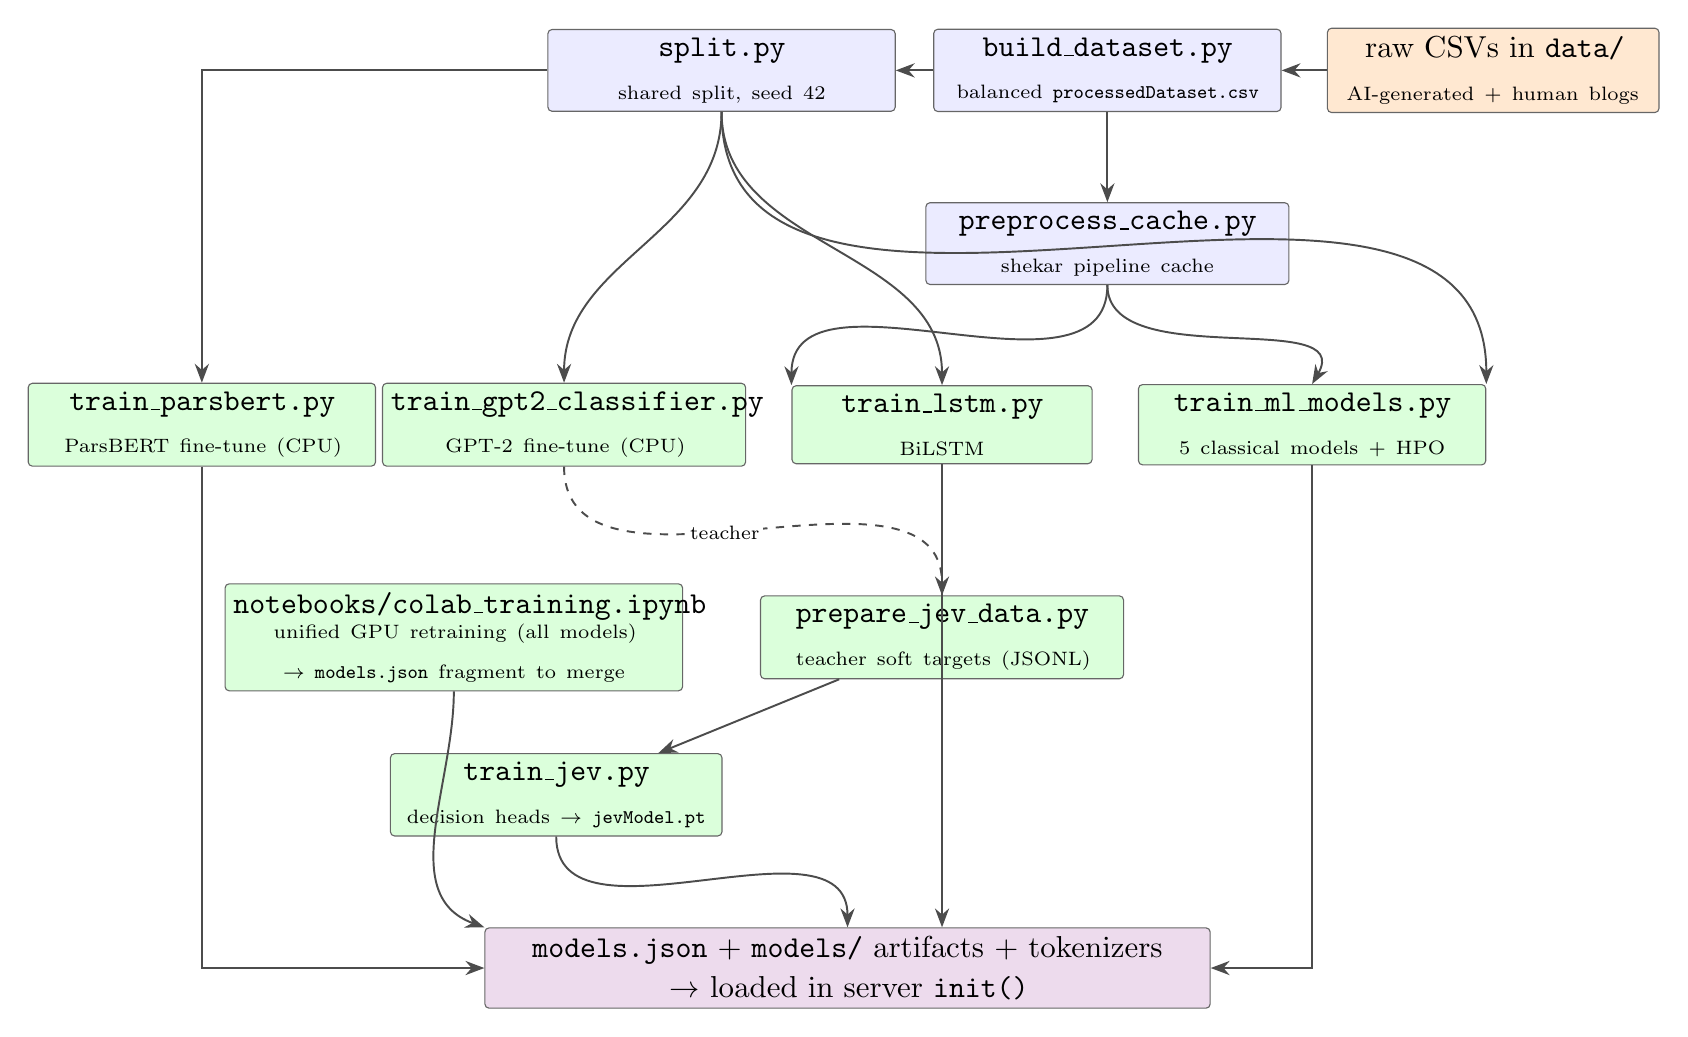
\begin{tikzpicture}
  % dataset build chain
  \node[data, w=4.0cm] (raw) at (0,0)
      {raw CSVs in \texttt{data/}\\[1pt]\scriptsize AI-generated + human blogs};
  \node[box, w=4.2cm] (bld) at (-4.9,0)
      {\texttt{build\_dataset.py}\\[1pt]\scriptsize balanced \texttt{processedDataset.csv}};
  \node[box, w=4.2cm] (sp) at (-9.8,0)
      {\texttt{split.py}\\[1pt]\scriptsize shared split, seed \en{42}};
  \node[box, w=4.4cm] (pc) at (-4.9,-2.2)
      {\texttt{preprocess\_cache.py}\\[1pt]\scriptsize \en{shekar} pipeline cache};
  % local CPU trainings
  \node[proc, w=4.2cm] (t1) at (-2.3,-4.5)
      {\texttt{train\_ml\_models.py}\\[1pt]\scriptsize 5 classical models + HPO};
  \node[proc, w=3.6cm] (t2) at (-7.0,-4.5)
      {\texttt{train\_lstm.py}\\[1pt]\scriptsize \en{BiLSTM}};
  \node[proc, w=4.4cm] (t3) at (-11.8,-4.5)
      {\texttt{train\_gpt2\_classifier.py}\\[1pt]\scriptsize \en{GPT-2} fine-tune (CPU)};
  \node[proc, w=4.2cm] (t4) at (-16.4,-4.5)
      {\texttt{train\_parsbert.py}\\[1pt]\scriptsize \en{ParsBERT} fine-tune (CPU)};
  \draw[arr] (raw) -- (bld);
  \draw[arr] (bld) -- (sp);
  \draw[arr] (bld.south) to[out=-90,in=90] (pc.north);
  \draw[arr] (sp.south) to[out=-90,in=90] (t1.north east);
  \draw[arr] (sp.south) to[out=-90,in=90] (t2.north);
  \draw[arr] (sp.south) to[out=-90,in=90] (t3.north);
  \draw[arr] (sp.west) -| (t4.north);
  \draw[arr] (pc.south) to[out=-90,in=60] (t1.north);
  \draw[arr] (pc.south) to[out=-90,in=90] (t2.north west);
  % unified GPU notebook
  \node[proc, w=5.6cm] (nb) at (-13.2,-7.2)
      {\texttt{notebooks/colab\_training.ipynb}\\[1pt]\scriptsize unified \en{GPU} retraining (all models)\\
       \scriptsize $\to$ \texttt{models.json} fragment to merge};
  % JEV line: teacher -> soft targets -> training
  \node[proc, w=4.4cm] (jd) at (-7.0,-7.2)
      {\texttt{prepare\_jev\_data.py}\\[1pt]\scriptsize teacher soft targets \en{(JSONL)}};
  \node[proc, w=4.0cm] (t5) at (-11.9,-9.2)
      {\texttt{train\_jev.py}\\[1pt]\scriptsize decision heads $\to$ \texttt{jevModel.pt}};
  \draw[arrd] (t3.south) to[out=-90,in=90] node[lbl, pos=0.45] {teacher} (jd.north);
  \draw[arr] (jd) -- (t5);
  % final artifacts
  \node[art, w=9.0cm] (art) at (-8.2,-11.4)
      {\texttt{models.json} + \texttt{models/} artifacts + tokenizers\\$\to$ loaded in server \texttt{init()}};
  \draw[arr] (t1.south) |- (art.east);
  \draw[arr] (t2.south) -- (t2.south |- art.north);
  \draw[arr] (t4.south) |- (art.west);
  \draw[arr] (nb.south) to[out=-90,in=160] (art.north west);
  \draw[arr] (t5.south) to[out=-90,in=90] (art.north);
\end{tikzpicture}}%
\caption{زنجیرهٔ بازتولید: از منابع خام تا آرتیفکت‌های سرویس. چهار آموزش
محلی سمت راست مستقل و روی پردازندهٔ مرکزی اجراشدنی‌اند؛ نوت‌بوک یکپارچهٔ
\en{Colab} (پایین چپ) همهٔ مدل‌ها را با \en{GPU} بازآموزی و قطعه‌ای برای
ادغام در \texttt{\lr{models.json}} تولید می‌کند. پیکان نقطه‌چین «معلم»،
مصرف خروجی دسته‌بند \en{GPT-2} برای ساخت هدف‌های نرم بخش~\ref{sec:jev}
است.}
\label{fig:training-flow}
\end{figure}

اسکریپت مستقل \texttt{\lr{eval\_perplexity.py}} نیز ارزیابی
بخش~\ref{sec:perplexity-signal} را بازتولید می‌کند.

هر سطر خروجی \texttt{\lr{prepare\_jev\_data.py}} یک رکورد \en{JSONL} به
سبک \en{Valen} است: «وضعیت» (متن)، شمای سه سؤال نوع‌بندی‌شده، و هدف‌های
نرم تقطیرشده از معلم. ساختار هر رکورد (مقادیر متنی نمونه خلاصه شده است):

\begin{LTRverb}
\begin{verbatim}
{
  "id": "train-000014",
  "split": "train",
  "label": 1,
  "state": {"text": "<full sample text>"},
  "teacher": "gpt2_transformer",
  "questions": {
    "source":       {"type": "choice",
                     "candidates": ["human_written", "ai_generated"]},
    "ai_level":     {"type": "score",
                     "levels": ["definitely_human", "probably_human",
                                "mixed_signals", "probably_ai",
                                "definitely_ai"]},
    "needs_review": {"type": "noul"}
  },
  "targets": {
    "source":       {"human_written": 0.02, "ai_generated": 0.98},
    "ai_level":     [0.0045, 0.0521, 0.2565, 0.4336, 0.2533],
    "needs_review": 0.0
  },
  "teacherAiProbability": 0.9968
}
\end{verbatim}
\end{LTRverb}

پس از آموزش، چک‌پوینت \texttt{\lr{jevModel.pt}} به‌همراه آستانه‌های سیاست
تصمیم ذخیره می‌شود و ورود \texttt{\lr{jev\_system\_one}} به فایل
\texttt{models.json} به‌طور خودکار نوشته می‌شود؛ با بازراه‌اندازی سرور،
مدل در رابط وب قابل انتخاب است.

\section{اجرای سرویس بک‌اند}
سرور از ریشهٔ پروژه و با محیط مجازی فعال اجرا می‌شود:
\begin{LTRverb}
\begin{verbatim}
# serve on 0.0.0.0:8000 (loads all artifacts at startup)
.venv/bin/python server.py

# or, during development, with live reload:
.venv/bin/uvicorn aitextd.api:app --reload --port 8000
\end{verbatim}
\end{LTRverb}
راه‌اندازی، همهٔ مدل‌ها، بردارساز و توکن‌سازها را یک‌بار بار و گرم می‌کند
(شکل~\ref{fig:inference-flow})؛ بنابراین نخستین پاسخ هم سریع است و هزینهٔ
بارگذاری سرد به درخواست کاربر منتقل نمی‌شود. صحت اجرا با فراخوانی فهرست
مدل‌ها بررسی می‌شود؛ پاسخ باید ۱۰ مدخل داشته باشد: ۹ مدل واقعی و «مدل
ترکیبی» در رأس فهرست:
\begin{LTRverb}
\begin{verbatim}
curl -s http://localhost:8000/models

# sample detection request (modelId can be any id from /models):
curl -s -X POST http://localhost:8000/detect \
  -H "Content-Type: application/json" \
  -d '{"text": "<a Persian sample of at least 20 chars>",
       "modelId": "ensemble"}'
\end{verbatim}
\end{LTRverb}

\section{اجرای رابط کاربری وب}
رابط وب در پوشهٔ \texttt{\lr{web-app/}} اجرا می‌شود:
\begin{LTRverb}
\begin{verbatim}
cd web-app
pnpm install
pnpm dev        # serves on http://localhost:3000
\end{verbatim}
\end{LTRverb}
یک نکتهٔ پیکربندی مهم: در نسخهٔ کنونی، مسیرهای پروکسی سمت سرور نشانی
بک‌اند را ثابت روی \texttt{\lr{0.0.0.0:8000}} فرض می‌کنند؛ پس سرور پایتون
باید روی همین درگاه در حال اجرا باشد (محدودیت شناخته‌شدهٔ فعلی و کاندیدای
طبیعی برای پارامتری‌شدن با متغیر محیطی). پس از اجرا، آدرس
\texttt{\lr{localhost:3000}} در مرورگر باز می‌شود؛ صحت اتصال با ارسال یک
متن حداقل ۲۰کاراکتری و دیدن نتیجهٔ تشخیص و جزئیات تحلیلی بررسی می‌شود.
تنظیمات سرویس آنلاین \en{TypeSafe} (نشانی پایه، نام مدل و کلید) از پنل
صفحهٔ اصلی وارد و فقط در \texttt{\lr{localStorage}} مرورگر ذخیره می‌شود
(بخش~\ref{sec:online-systemone}).

\section{آزمون‌های خودکار}
مجموعهٔ آزمون از ریشهٔ پروژه اجرا می‌شود:
\begin{LTRverb}
\begin{verbatim}
.venv/bin/python -m pytest tests/ -m "not slow"   # fast behavior tests
.venv/bin/python -m pytest tests/ -m slow         # full stack + golden
\end{verbatim}
\end{LTRverb}
آزمون‌های سریع، منطق خالص (پیش‌پردازش، ویژگی‌های سبکی، معماری مدل‌ها و
بسته‌بندی پاسخ \en{JEV}) را بدون نیاز به چک‌پوینت می‌آزمایند؛ آزمون با نشان
\en{slow}، کل پشتهٔ سرویس را بار می‌کند و خروجی دقیق
\texttt{\lr{detection()}} را با مقادیر ثبت‌شده در
\texttt{\lr{tests/golden/detection\_golden.json}} مقایسه می‌کند: در نخستین
اجرا خروجی‌ها ثبت و سپس قفل می‌شوند و هر تغییری که یک پیش‌بینی
سرویس‌شده را عوض کند، مجموعهٔ آزمون را شکست می‌دهد — همان سازوکاری که
ناهم‌خوانی آموزش/سرویس (بخش~\ref{sec:style-features}) را پس از هر
بازآموزی آشکار می‌سازد.

\section{افزودن یک مدل تازه به سرویس}
برای مدلی که از یکی از مقادیر شناخته‌شدهٔ \texttt{runtime} (جدول~\ref{tab:runtimes})
پیروی می‌کند، تنها دو گام لازم است: (۱) ذخیرهٔ آرتیفکت با نام فایل
ثبت‌شده در پوشهٔ \texttt{\lr{models/}}، و (۲) افزودن مدخل آن به
\texttt{\lr{models.json}} با فیلدهای \texttt{\lr{id}}،
\texttt{\lr{runtime}}، \texttt{\lr{filename}}،
\texttt{\lr{ensembleWeight}} و معیارهای ارزیابی؛ سپس راه‌اندازی مجدد سرور.
نقاط پایانی \en{API} و رابط وب هیچ تغییری لازم ندارند — همان مزیت اعزام
زمان اجرا که افزودن \en{GPT-2}، \en{ParsBERT} و \en{JEV} را بدون تغییر
معماری ممکن کرد. افزودن یک مقدار \texttt{runtime} تازه (چنان‌که برای
\texttt{\lr{pytorch-parsbert}} و \texttt{\lr{pytorch-jev}} رخ داد) نیز
تنها به یک جفت تابع بارگذار/پیش‌بین نیاز دارد که در
\texttt{\lr{aitextd/loaders.py}} و \texttt{\lr{aitextd/predictors.py}} به
نگاشت‌های زمان اجرا افزوده می‌شوند.

% =============================================================================
% ۸) مراجع
% =============================================================================
\clearpage
\phantomsection
\addcontentsline{toc}{chapter}{مراجع}
\begin{thebibliography}{99} % FIX: use 99 to be safe

\bibitem{vaswani2017attention}
\lr{A. Vaswani, N. Shazeer, N. Parmar, J. Uszkoreit, L. Jones, A. N. Gomez,
{\L}. Kaiser, I. Polosukhin.
\textit{Attention Is All You Need}.
Advances in Neural Information Processing Systems (NeurIPS), 2017.}

\bibitem{radford2019gpt2}
\lr{A. Radford, J. Wu, R. Child, D. Luan, D. Amodei, I. Sutskever.
\textit{Language Models are Unsupervised Multitask Learners}.
OpenAI Technical Report, 2019.}

\bibitem{hochreiter1997lstm}
\lr{S. Hochreiter, J. Schmidhuber.
\textit{Long Short-Term Memory}.
Neural Computation, 9(8):1735--1780, 1997.}

\bibitem{breiman2001randomforest}
\lr{L. Breiman.
\textit{Random Forests}.
Machine Learning, 45(1):5--32, 2001.}

\bibitem{friedman2001gbm}
\lr{J. F. Friedman.
\textit{Greedy Function Approximation: A Gradient Boosting Machine}.
Annals of Statistics, 29(5):1189--1203, 2001.}

\bibitem{salton1988tfidf}
\lr{G. Salton, C. Buckley.
\textit{Term-Weighting Approaches in Automatic Text Retrieval}.
Information Processing \& Management, 24(5):513--523, 1988.}

\bibitem{howard2018ulmfit}
\lr{J. Howard, S. Ruder.
\textit{Universal Language Model Fine-tuning for Text Classification}.
Proceedings of ACL, 2018.}

\bibitem{farahani2021parsbert}
\lr{M. Farahani, M. Gharachorloo, M. Farahani, M. Manthouri.
\textit{ParsBERT: Transformer-based Model for Persian Language Understanding}.
Neural Processing Letters, 53(6):3831--3847, 2021.}

\bibitem{hoosman-gpt2fa}
\lr{HooshvareLab.
\textit{gpt2-fa: A GPT-2 Language Model Pretrained on Persian Text}.
Hugging Face Model Hub, \url{https://huggingface.co/HooshvareLab/gpt2-fa}.}

\bibitem{torabifarsani2026dataset}
\lr{E. Torabi Farsani.
\textit{Persian AI-Generated Text Dataset}.
Hugging Face Datasets, 2026,
\url{https://huggingface.co/datasets/ehsantorabi/persian-ai-generated-text}.}

\bibitem{jev-typesafe}
\lr{TypeSafe.
\textit{Jev: A Practical Guide to System One Models and Typed AI}.
Hugging Face Blog, 2026,
\url{https://huggingface.co/blog/paidaxccc/jev-system-one-model-a-practical-guide-to-typed-ai}.}

\bibitem{valen2026}
\lr{Liuziyu77.
\textit{Valen: An Open-Source Multimodal Decision Model Inspired by Jev}.
GitHub Repository, 2026,
\url{https://github.com/Liuziyu77/Valen}.}

\end{thebibliography}

\end{document}
